\documentclass[a4paper,10pt,hidelinks]{book}

\usepackage{kotex}
\usepackage[open,openlevel=1,numbered]{bookmark}
\usepackage[fleqn]{amsmath}
\usepackage{xcolor}

\usepackage{minitoc}

\nomtcrule
\renewcommand{\mtcindent}{2pt}
\renewcommand{\mtcfont}{\normalsize\rm}
\renewcommand{\mtcSfont}{\normalsize\rm}

\usepackage{setspace}
\usepackage{titlesec}

\titlespacing
    {\subsection} % command
    {0pt} % left
    {1.5\parskip} % before
    {-0.5\parskip} % after

\usepackage{geometry}

\setlength{\parindent}{0pt}
\setlength{\parskip}{8pt}
\linespread{1.6}
\geometry{
    top=2.5cm,
    bottom=2.5cm,
    left=2.2cm,
    right=2.2cm,
}

\usepackage{array}
\usepackage{multirow}
\usepackage{makecell}
\usepackage{colortbl}

\definecolor{tblheadcolor}{HTML}{DFE6F7}

\newcommand\colc\centering
\newcommand\coll\raggedright
\newcommand\colr\raggedleft
\newcommand\tw\textwidth

\newlength{\thickarrayrulewidth}
\setlength{\thickarrayrulewidth}{2.0\arrayrulewidth}
\renewcommand{\arraystretch}{2.0}
\setlength\extrarowheight{-1pt}

\makeatletter
\def\thickhline{%
    \noalign{\ifnum0=`}\fi\hrule \@height \thickarrayrulewidth \futurelet
        \reserved@a\@xthickhline}
\def\@xthickhline{\ifx\reserved@a\thickhline
                \vskip\doublerulesep
                \vskip-\thickarrayrulewidth
                \fi
                \ifnum0=`{\fi}}
\makeatother

\newcolumntype{?}{!{\vrule width 1.6pt}}

\newenvironment{tblenv}[3]
    {\vspace{15pt}\begin{table}[htb]
        \centering
        \caption{#2\label{#1}}
        \small\begin{tabular}{#3}\thickhline}
    {\thickhline\end{tabular}\vspace{15pt}\end{table}}

\usepackage{graphicx}
\usepackage{subcaption}
% \usepackage{floatrow}
% \usepackage[label font=bf,labelformat=simple]{subfig}

% \floatsetup[figure]{style=plain,subcapbesideposition=top}

\newcommand{\figcmd}[4]{
    \begin{figure}[htb]
        \vspace{10pt}\centering
        \includegraphics[scale=#4]{#3}
        \caption{#2 \label{#1}}
    \end{figure}
}

\usepackage{amsthm}
\usepackage{mdframed}
\usepackage{fancyvrb}

\newcommand\cd\texttt

\definecolor{codebgcolor}{HTML}{E7E7E7}

\mdfdefinestyle{codeframe}{
    hidealllines=true,
    backgroundcolor=codebgcolor,
    innertopmargin=-3pt,
    innerbottommargin=8pt,
}

\makeatletter
\def\thmhead@plain#1#2#3{%
    \thmname{#1}\thmnumber{\@ifnotempty{#1}{ }\@upn{#2}}%
    \thmnote{ {\the\thm@notefont#3}}}
\let\thmhead\thmhead@plain
\makeatother

\newtheoremstyle{codestyle}% name of the style to be used
    {20pt}% measure of space to leave above the theorem. E.g.: 3pt
    {}% measure of space to leave below the theorem. E.g.: 3pt
    {}% name of font to use in the body of the theorem
    {}% measure of space to indent
    {\bfseries}% name of head font
    {}% punctuation between head and body
    {0pt}% space after theorem head
    {}% Manually specify head
\theoremstyle{codestyle}

\newtheorem{code}{Code}[chapter]
\newenvironment{codeenv}[2]
    {\vspace{10pt}\begin{mdframed}[style=codeframe]\begin{code}[#2]\label{#1}\linespread{1.1}{\ }}
    {\end{code}\end{mdframed}\vspace{6pt}}

\newtheorem{shell}{Shell}[chapter]
\newenvironment{shellenv}[2]
    {\vspace{10pt}\begin{mdframed}[style=codeframe]\begin{shell}[#2]\label{#1}\linespread{1.1}{\ }}
    {\end{shell}\end{mdframed}\vspace{6pt}}

\newtheorem{sql}{SQL}[chapter]
\newenvironment{sqlenv}[2]
    {\vspace{10pt}\begin{mdframed}[style=codeframe]\begin{sql}[#2]\label{#1}\linespread{1.1}{\ }}
    {\end{sql}\end{mdframed}\vspace{6pt}}

% \newcounter{exercise}[chapter]
\renewcommand{\theexercise}{\thechapter.\arabic{exercise}}

\addtocounter{exercise}{1}
\newcommand{\excref}[1]{Exercise \ref{#1}}
\newcommand{\excstref}[1]{\refstepcounter{exercise}Exercise \theexercise\label{#1}}

\usepackage{caption}

\newcommand{\chapref}[1]{\ref{#1}장}
\newcommand{\sectref}[1]{\ref{#1}절}
\newcommand{\figref}[1]{\textbf{Figure \ref{#1}}}
\newcommand{\tblref}[1]{\textbf{Table \ref{#1}}}
\newcommand{\coderef}[1]{\textbf{Code \ref{#1}}}
\newcommand{\shellref}[1]{\textbf{Shell \ref{#1}}}
\newcommand{\sqlref}[1]{\textbf{SQL \ref{#1}}}

\renewcommand{\contentsname}{Table of Contents}

\captionsetup{
    format=hang,
    font=small,
    labelfont=bf,
    labelsep=space,
}

\captionsetup[table]{
    justification=centering,
    singlelinecheck=false,
}

\usepackage{enumitem}

\setlist[itemize]{
    itemsep=-5pt,
    topsep=-3pt,
}

\setlist[enumerate]{
    itemsep=-5pt,
    topsep=-3pt,
}


\begin{document}
    \begin{titlepage}
    \centering
    \vspace*{35mm}
    \fig{images/kweb-logo.png}{0.1}
    \par\vspace{5mm}
    {\large KWEB, Korea University}
    \par\vspace{20mm}
    {\large\bfseries 2021 Web Application Essentials \par\huge Backend Section}
    \par\vspace{30mm}
    {\large Written By: Lee, Chanyoung}
    \par\vspace{30mm}
    {\large October 20, 2021}
\end{titlepage}

    \dominitoc
    \tableofcontents

    \chapter{Introduction to Front-end}\label{ch:intoduction-to-front-end}
    \minitoc
    \section{Introducing WEB} \label{sect:introducing-web}

\subsection*{WEB}
웹(WEB)이란, 인터넷에 연결된 컴퓨터들을 통해 사람들이 정보를 공유할 수 있는 전 세계적인 정보 공간이다. 웹을 통해 공유되는 정보들은 대개 웹 페이지(web page)의 형태로 공유되며, 웹 페이지는 특수한 양식을 갖춘 텍스트로 구성된다. 각 웹페이지는 일반적인 텍스트(plain text)뿐만 아니라 이미지, 동영상, 다른 웹페이지로 연결되는 하이퍼링크(hyperlink) 등의 웹 자원(web resource)으로 다양하게 구성되고, 하나의 주제, 하나의 영역을 공유하는 여러 웹 자원과 웹 페이지는 웹 사이트(website)를 구성한다. 웹 사이트는 웹 서버(web server)라는 디바이스에서 동작하는 웹 애플리케이션(web application)이라고 하는 프로그램에 의해 구현되어 작동하며, 이 웹 애플리케이션으로 인해 권한만 충분하다면 전 세계 어디서든 웹 사이트에 접속할 수 있다.

본 교재에서 다루는 웹의 영역은 웹 애플리케이션과 관련된 영역이며, 흔히 웹 개발자가 다루는 웹의 영역도 이와 상당수 일치한다. 앞으로 여러분은 웹 애플리케이션의 작동 원리와 구조를 이해하고, HTML과 CSS, Javascript를 이용하여 웹을 디자인하고 설계하는 학습을 할 것이다.

\subsection*{Front-end and Back-end}
웹 서버, 혹은 웹 사이트가 작동하는 원리를 생각해보자. 예를 들어, 사용자가 블로그 형태의 웹 사이트에 접속했을 때 사용자에게 보여지는 영역에는 어떤 것이 있는가? 블로그의 블로거, 블로거에 대한 상세 정보, 게시물, 게시물에 대한 상세 정보, 댓글, 댓글에 대한 상세 정보 등이 있을 것이다. 뿐만 아니라 블로그를 예쁘게 꾸민 디자인 등도 사용자에게 보여지는 영역이다. 이렇듯 사용자에게 보여지는 영역을 \textbf{front-end}라고 부르며, 사용자(client) 쪽에서 동작하는 영역이라고 하여 \textbf{client-side}라고도 부른다.

반대로, 사용자에게 직접적으로 보여지지 않는 영역도 있다. 사용자의 요청에 맞게 적절한 웹 페이지를 구성하여 전달해주는 로직, 게시물이나 댓글, 블로거의 정보를 데이터베이스에 저장하고 데이터베이스로부터 읽어오는 기능, 회원에 따라 글을 작성할 권한을 부여할 것인지, 댓글을 수정할 권한을 부여할 것인지 결정하는 로직 등이 있을 것이다. 이렇게 사용자에게 직접적으로 보여지지 않는 영역을 \textbf{back-end}라고 부르고, 이러한 로직은 서버상에서 동작하기 때문에 \textbf{server-side}라고도 부른다.

\figures{fig:webapp-schema}{How Typical Web Application Works}
    {\fig{images/introduction-to-front-end/webapp-schema.png}{.6}}

본 교재에서는 front-end 분야를 다루며, front-end에서 기본적으로 사용되는 HTML, CSS, Javascript를 학습한다. 이를 응용하여 실무에서는 React.js, Vue.js, Angular.js 등의 프레임워크를 사용하기도 한다.

    \section{2021 Study Schedule} \label{sect:2021-study-schedule}

\subsection*{스터디 일정}
\begin{tblenv}
    {tab:frontend-study-schedule}
    {2021 Front-end Study Schedule}
    {
        >{\centering}m{0.04\textwidth}
        >{\centering}m{0.15\textwidth}
        >{\raggedright}m{0.5\textwidth}
        >{\raggedright}m{0.2\textwidth}
    }
    \thickhline
    회차 & 스터디 날짜 & 스터디 내용 & 비고 \tabularnewline
    \hline
    1 & 03/29 \textasciitilde 04/02 & Intro. to Front-end, HTML: The Basic Structure &  \tabularnewline
    2 & 04/05 \textasciitilde 04/09 & HTML: The Basic Structure, CSS: Designing HTML & 중간고사 이전 회차 \tabularnewline
    3 & 05/03 \textasciitilde 05/07 & CSS: Designing HTML & 중간고사 이후 회차 \tabularnewline
    4 & 05/10 \textasciitilde 05/14 & CSS: Designing HTML &  \tabularnewline
    5 & 05/17 \textasciitilde 05/21 & Basics of Javascript &  \tabularnewline
    6 & 05/24 \textasciitilde 05/28 & JS: Dynamic Frontend &  \tabularnewline
    7 & 05/31 \textasciitilde 06/04 & JS: Dynamic Frontend & 기말고사 이전 회차 \tabularnewline
    \thickhline
\end{tblenv}

\subsection*{OUT COUNT 제도}
준회원 스터디 과정에서는 3 OUT COUNT 제도가 시행되며, OUT COUNT는 다음과 같은 경우에 적용된다.
\begin{itemize}
    \item 0.5 OUT : 스터디 사유 불참, 스터디 무단 지각, 과제 지각 제출
    \item 1.0 OUT : 스터디 무단 불참, 과제 미제출
    \item 2.0 OUT : 과제 Cheating
\end{itemize}
스터디 지각은 스터디 시작 이후 15분까지만 가능하며, 과제 지각 제출은 과제 제출 기한 이후 3일 이내에만 받는다. OUT COUNT가 3.0을 초과하면 본 스터디의 Pass 자격이 박탈될 수 있다.

\subsection*{평가 시험}
본 스터디는 평가 시험에 통과하여야 Pass할 수 있으며, 본 스터디를 Pass하여야 Back-end 스터디에 참여할 수 있다. 평가 시험은 KWEB 종강총회 당일에 치뤄지며, 종강총회는  일정은 KWEB 종강총회 당일이며, 종강총회는 6/19(토)로 예정되어 있다. 평가 시험은 약 60분간 진행되며, 일정 점수 이상 취득하여야 통과할 수 있고, 통과하지 못하였거나 응시하지 않은 경우 여름방학에 보충 스터디\footnote{열리지 않을 수도 있음.}에 참여하여야 Back-end 스터디에 참여할 수 있다.

    \section{Setting Development Environment} \label{sect:setting-development-environment}

\subsection*{Visual Studio Code}
웹 개발을 보다 간편하게 할 수 있도록 개발 환경을 구축해보자. 준회원 스터디에서는 널리 이용되는 소스 코드 편집기인 Visual Studio Code를 사용한다. 물론, Atom이나 Vim 등 본인이 더 선호하는 편집기가 있다면 사용하여도 무관하나, 사용 과정에서 문제가 발생했을 때 도움을 제공하기는 힘들다는 점을 미리 말해둔다.

VS Code 홈페이지인 https://code.visualstudio.com/\#alt-downloads에 접속하여 본인의 운영체제에 맞게 설치한다.

\subsection*{Chrome / Firefox}
Chrome과 Firefox는 널리 사용되는 대표적인 인터넷 브라우저이다. Internet Explorer 역시 널리 알려진 인터넷 브라우저이나, 지속적으로 업데이트되는 웹 표준을 제때 따라오지 못해 개발 시에 다소 어려움을 유발하고, Chrome이나 Firefox가 더 편리한 디버깅 도구를 제공하므로 Chrome이나 Firefox를 사용하는 것을 권장한다.


    \chapter{HTML: The Basic Structure}\label{ch:html-the-basic-structure}
    \minitoc
    \section{Introducing HTML} \label{sect:introducing-html}

HTML은 HyperText Markup Language의 약자로, 웹 브라우저에 웹 페이지의 구조를 체계적으로 표현하는 컴퓨터 언어이다. HTML은 웹 페이지의 가장 기본적인 뼈대를 이루며, 어떤 front-end framework를 사용하던 HTML을 필수적으로 이해하고 있어야 한다.

\subsection*{HTML is not a Programming Language?}

소프트웨어 개발과 관련된 밈(meme)을 접하다 보면 가장 자주 듣는 밈 중 하나가 바로 ``HTML is not a programming language'', 즉 HTML은 프로그래밍 언어가 아니라는 밈이다. 실제로 HTML은 프로그래밍 언어가 아닌, 구조를 서술하기 위한 언어로, 쉽게 접할 수 있는 프로그래밍 언어인 C, Java, Python 등과 달리 조건문, 반복문, 변수 선언 등의 기능이 전혀 없다. 구조를 서술하기 위해 존재하는 언어이니만큼, \textbf{미리 정해진 규칙}에 따라 HTML을 작성하여 \textbf{구조를 표현}한다는 개념으로 접근하면 HTML이라는 언어에 대해 감을 잡을 수 있을 것이다.

\figures{fig:html-not-pl}{HTML is not a programming language}
    {\fig{images/html-the-basic-structure/html-is-not-a-programming-language.png}{.5}}

    \section{Basic Structure of HTML} \label{sect:basic-structure-of-html}

\subsection*{Tags and Elements}
HTML은 HyperText Markup Language의 약자로, 마크업 언어의 일종이다. 마크업 언어란, HTML은 마크업 언어이며, 마크업 언어는 구조를 서술할 때 정해진 마크로 시작하여 마크로 끝나는 언어이다. \coderef{code:html-ex}를 보며 이해해보자.

\begin{codeenv}{code:html-ex}{Example of HTML}\begin{verbatim}


<!doctype html>
<html>
<head>
    <title>Example Domain</title>

    <meta charset="utf-8" >
    <meta http-equiv="Content-type" content="text/html; charset=utf-8" >
    <meta name="viewport" content="width=device-width, initial-scale=1" >
</head>

<body>
    <div>
        <h1>Example Domain</h1>
    </div>
</body>
</html>
\end{verbatim}
\end{codeenv}

\coderef{code:html-ex}을 관찰해보자. Example Domain이라는 내용을 \verb|<title>|과 \verb|</title>|이 감싸고 있는데, 이러한 문자열을 태그(tag)라고 한다. 두 태그에서 \verb|title|을 \textbf{태그 이름(tag name)}이라고 하며, 태그 내부의 내용(Example Domain)을 태그의 \textbf{내용(content)}이라고 한다. 슬래시(\verb|/|)가 붙어있어 뒤쪽에 오는 태그를 끝 태그(end tag)라고 한다. 유사하게, 이 \verb|title| 태그를 \verb|<head>|와 \verb|</head>|가 감싸고 있는 것을 확인할 수 있다. 이처럼 HTML은 기본적으로 내용의 양 끝단을 태그로 감쌈으로써 구조를 표현한다. 다만, \verb|meta| 태그와 같이 end tag가 존재하지 않는, 단일 태그도 존재한다. 이렇게 태그와 그 태그 사이에 wrap 되어있는 내용이 하나의 \textbf{HTML 요소(element)}를 구성한다.\footnote{단일 태그는 그 자체만으로 하나의 요소가 된다.}

\coderef{code:html-ex}을 더 깊게 관찰해보면, \verb|head| 태그의 요소와 \verb|body| 태그의 요소가 \verb|html| 태그의 요소 일부분인 것을 확인할 수 있다. 즉, HTML 요소는 내부에 또 다른 HTML 요소를 포함할 수 있고, 다른 HTML 요소의 일부가 될 수 있으며, 이와 같은 구조를 nested 구조라고 한다. HTML에서는 요소 A가 요소 B의 일부분을 구성할 때, 요소 A를 요소 B의 \textbf{하위 요소(sub element) 혹은 자식 요소(child element)}라고 하고, 요소 B를 요소 A의 \textbf{상위 요소(super element) 혹은 부모 요소(parent element)}라고 한다.

\figcmd{fig:html-elmt-struct}{Structure of HTML Element}
    {images/html-the-basic-structure/html-elmt-struct.png}{.7}

이제까지 살펴본 HTML 요소의 구조를 종합해보면 \figref{fig:html-elmt-struct}와 같이 표현할 수 있다. 태그의 이름은 대소문자를 구별하지 않으나 소문자로 쓰는 것이 원칙이다. 각 요소에는 속성(attribute)을 설정해줄 수 있으며, 이 경우 속성의 이름과 그에 대응하는 값(value)을 태그에 같이 써줍니다. HTML 요소의 속성은 태그나 내용 못지않게 중요한 역할을 하는데, \sectref{sect:commonly-used-html-tags}에서 더 자세히 알아보도록 하자.

\subsection*{HTML의 기본적인 구조}
HTML 문서의 구조에는 가장 기본적인 틀이 정해져 있다. 먼저 \verb|doctype|을 이용하여 문서가 HTML 문서임을 명시히고, 가장 상위 태그로 \verb|html| 태그, 그 아래에 \verb|head|와 \verb|body| 태그가 위치해야 한다. 코드로 나타낸다면 \coderef{code:html-basic-struct}와 같다.\footnote{HTML에서는 주석을 \texttt{<!--}, \texttt{-->}로 표현한다.}

\begin{codeenv}{code:html-basic-struct}{Basic Structure of HTML}
\begin{verbatim}


<!doctype html>
<html>
    <head>
        <!-- Head Element Content -->
    </head>

    <body>
        <!-- Body Element Content -->
    </body>
</html>
\end{verbatim}
\end{codeenv}

\verb|head| 태그는 문서에 대한 전반적인 정보를 담고 있는 태그로, 이 태그에는 \verb|title|, \verb|meta|, \verb|link| 등 다양한 태그들이 사용되나, 가장 대표적인 두 태그만 살펴보자. 먼저, \verb|title| 태그 내부의 텍스트는 웹 페이지의 제목으로, 웹 브라우저를 통해 웹 페이지에 접속했을 때 브라우저의 상단에 표시된다. \verb|meta| 태그는 HTML 문서의 인코딩 방법, viewport, 키워드 등 중요한 정보들을 지정할 수 있는 태그이다. 

\verb|body| 태그는 웹 페이지에서 사용자에게 보여질 부분이 포함되는 태그이다. 개발자가 웹 페이지를 통해 사용자에게 보여주고자 하는 텍스트, 이미지 등의 내용은 \verb|body| 태그 안에 구현되어야 하며, \sectref{sect:commonly-used-html-tags}에서 본격적으로 웹 페이지의 내용을 구현하는 방법에 대한 학습을 진행한다.

    \section{Commonly Used HTML Tags} \label{sect:commonly-used-html-tags}

이 절에서는 소개되는 태그들은 HTML에서 굉장히 자주 사용되는 태그들이다. 예제를 따라서 직접 작성해보고 웹 브라우저에서 열어 결과를 확인해보자.

\subsection*{Heading (\texttt{h1} - \texttt{h6}) Tags}
\texttt{h1} - \texttt{h6} 태그는 heading의 약자로, 제목을 나타낼 때 사용되는 태그이다. h 뒤의 숫자가 작을수록 화면에 표시되는 글자의 크기가 크다. \coderef{code:heading-tags}을 직접 실행해보고, 태그 내부의 내용을 바꾸어보자.

\begin{codeenv}{code:heading-tags}{\texttt{h1} - \texttt{h6} Tags}\begin{verbatim}


<h1>This is h1 tag</h1>
<h2>This is h2 tag</h2>
<h3>This is h3 tag</h3>
<h4>This is h4 tag</h4>
<h5>This is h5 tag</h5>
<h6>This is h6 tag</h6>
\end{verbatim}
\end{codeenv}

\subsection*{\texttt{p}, \texttt{br} Tag}
\texttt{p} 태그는 paragraph의 약자로, 문단을 구분해주는 태그이다. 이 태그는 문단과 문단 사이에 공백을 넣어주는 역할을 하며, 문단과 문단의 사이에는 별도의 공간이 생긴다. 

HTML에서는 공백( ), 줄 바꿈(\verb|\n|) 등의 whitespace 문자들은 종류와 관계없이 하나의 공백 취급을 받고, 이러한 whitespace 문자들은 여러 개 연속적으로 나열되어도 하나의 공백으로 취급된다. 따라서, 코드 내에서 줄 바꿈을 하여 작성해도 실제로는 줄 바꿈이 되지 않으며, 줄 바꿈을 하기 위해서는 \texttt{br} 태그를 줄 바꿈 하고자 하는 위치에 넣어야 한다. 

\begin{codeenv}{code:par-tag}{\texttt{p}, \texttt{br} Tag}\begin{verbatim}


<p>
    HTML stands for HyperText Markup Language.<br>
    It is a language used to express the structure of webpage.
</p>
<p>
    Languages used to implement client-side are HTML, CSS and Javascript.<br>
    HTML and CSS are not programming languages, but Javascript is. <br>
</p>
\end{verbatim}
\end{codeenv}

\subsection*{\texttt{a} Tag}
\texttt{a} 태그는 HTML 요소에 다른 웹 페이지로 이동할 수 있는 하이퍼링크를 걸 수 있는 태그이다. 이 태그는 속성값에 유의하여 작성하여야 하며, 다음 세 속성은 \texttt{a} 태그에서 가장 자주 쓰이는 속성들이다. 

\begin{itemize}
    \item \texttt{href}: HTML 요소와 연결될 리소스의 주소
    \item \texttt{title}: HTML 요소와 연결될 리소스에 대한 설명. 호버(마우스를 위에 갖다 대는 것)를 했을 때 표시됨.
    \item \texttt{target}: 문서가 로드될 대상을 지정하는 옵션
        \begin{itemize}
            \item \texttt{\_blank}: 새로운 창이나 탭
            \item \texttt{\_self}: 현재 창
            \item \texttt{\_parent}, \texttt{\_top}: 잘 쓰이지 않는 옵션
        \end{itemize}
\end{itemize}

\coderef{code:atag}를 직접 실행해보고, 위의 속성값을 참고하여 \texttt{a} 태그를 활용해보자.

\begin{codeenv}{code:atag}{\texttt{a} Tag}\begin{verbatim}


<a href="https://www.google.com" title="Google Homepage" target="_self">Google</a>
<br>
<a href="https://www.naver.com" title="Naver" target="_blank">Naver</a>
\end{verbatim}
\end{codeenv}

\subsection*{\texttt{button} Tag}
\texttt{button} 태그는 클릭할 수 있는 버튼을 생성하는 태그이다. 이 태그를 눌렀다가 놓았을 때 특정한 동작이 수행될 수 있으며, \texttt{input} 태그를 이용해서도 유사한 기능을 구현할 수는 있으나 디자인적 관점에서 \texttt{button} 태그가 더 편하므로 더 많이 사용한다. 

\texttt{button} 태그에 중요한 속성으로는 \texttt{disabled}, \texttt{type} 등이 있다. \texttt{disabled} 속성을 설정하면 버튼은 비활성화되어 클릭할 수 없는 상태가 되며, \texttt{type}은 버튼을 눌렀을 때 수행되는 동작의 성격에 차이가 생긴다. 버튼을 눌렀을 때 동작이 수행되도록 하는 방법은 \chapref{ch:javascript-dynamic-frontend}에서 다룬다.

\begin{codeenv}{code:button-tag}{\texttt{button} Tag}\begin{verbatim}


<button type="submit">Learn front-end</button>
<button disabled>Learn back-end</button>
\end{verbatim}
\end{codeenv}

\subsection*{List Tags}
리스트, 즉 항목들을 나열하여 표현할 수 있는 태그들이 세 가지 있다. 순서가 없는 리스트(unordered list)를 나타내는 \texttt{ul} 태그, 순서가 있는 리스트(ordered list)를 나타내는 \texttt{ol} 태그가 있으며, 두 종류의 리스트 모두 리스트의 각 원소를 \texttt{li} 태그를 이용하여 나열한다.

\texttt{ul} 태그나 \texttt{ol} 태그를 이용하여 리스트를 표현하면 각 원소의 앞에 bullet과 같은 문자나 숫자가 자동으로 생깁니다. 이러한 표식은 CSS를 활용하여 제거하거나 변경할 수 있다. \coderef{code:list-tags}을 직접 실행해보고, 다양한 형태의 리스트를 직접 만들어보자.

\begin{codeenv}{code:list-tags}{List Tags}\begin{verbatim}


<h3>Unordered List</h3>
<ul>
    <li>Visual Studio Code</li>
    <li>Atom</li>
    <li>Sublime Text</li>
    <li>Vim</li>
</ul>

<h3>Ordered List</h3>
<ol>
    <li>Visual Studio Code</li>
    <li>Atom</li>
    <li>Sublime Text</li>
    <li>Vim</li>
</ol>
\end{verbatim}
\end{codeenv}

\subsection*{\texttt{img} Tag}
\texttt{img} 태그는 HTML 문서에 이미지를 삽입할 수 있는 단일 태그이다. 다음은 \texttt{img} 태그에 사용되는 몇 가지 속성이다.

\begin{itemize}
    \item \texttt{src}: 삽입하고자 하는 이미지의 주소
    \item \texttt{alt}: 이미지를 가져오는 데 실패하였을 때 대신 표시되는 이미지에 대한 설명
    \item \texttt{width}: 이미지를 띄우고자 하는 너비 (px)
    \item \texttt{height}: 이미지를 띄우고자 하는 높이 (px)
\end{itemize}

\begin{codeenv}{code:img-tag}
    {\texttt{img} Tag\footnote{이 코드에서는 HTML의 속성-속성값 쌍을 분리하기 위해 1칸의 공백 대신 개행 문자와 5칸의 공백을 사용하였다. HTML에서는 연속된 whitespace 문자들을 하나의 공백으로 취급하기 때문에 이렇게 표시할 수 있으며, 속성이 많거나, 속성값이 길거나, 내용이 길거나 등의 이유로 HTML 요소가 지나치게 길어지면 이와 같이 개행하여 작성하는 것이 좋다.}}
    \begin{verbatim}


<img src="https://s.pstatic.net/static/www/img/uit/2019/sp_search.svg"
     alt="Naver Logo"
     width=640>
<img src="https://t1.daumcdn.net/daumtop_chanel/op/nonexist.png" alt="Daum Logo">
\end{verbatim}
\end{codeenv}

\subsection*{Font Tags}
글자의 폰트를 변경할 수 있는 태그들이다. 간단한 HTML 문서를 작성할 때는 쓰일 수 있으나, CSS를 활용하여 작성하는 것이 권장되기 때문에 자주 쓰이지는 않는다. 

\begin{codeenv}{code:font-tags}{Font Tags}\begin{verbatim}


<b>Bold Text</b><br>
<strong>Important Text</strong><br>
<i>Italic Text</i><br>
<em>Emphasized Text</em><br>
<mark>Marked Text</mark><br>
<small>Small Text</small><br>
<del>Deleted Text</del><br>
<ins>Inserted Text</ins><br>
<sub>Subscript</sub> Text<br>
<sup>Superscript</sup> Text<br>
\end{verbatim}
\end{codeenv}

\subsection*{Input Tags}
입력 태그들은 사용자로부터 정보를 입력받을 수 있는 태그들로, \texttt{input}, \texttt{textarea}, \texttt{select} 등의 태그가 있다. \texttt{input} 태그는 \texttt{type} 속성에 따라 다양한 형태의 입력을 받을 수 있다. 다음은 \texttt{input} 태그의 \texttt{type} 속성의 값에 따라 입력받을 수 있는 정보의 형태 중 일부를 나타낸 것이다.

\begin{itemize}
    \item \texttt{text}: 일반 텍스트 (plain text)
    \item \texttt{password}: 비밀번호
    \item \texttt{radio}: 선택 목록 중 하나만 선택할 수 있음
    \item \texttt{checkbox}: 선택 목록 중 여러 개 선택할 수 있음
\end{itemize}

\texttt{textarea} 태그는 \texttt{input} 태그와는 달리 여러 줄의 텍스트를 입력받을 수 있으며, 입력받는 부분의 크기나 설명 등은 속성을 이용하여 설정할 수 있다. \texttt{select}, \texttt{option} 태그는 여러 선택지 중 하나를 선택할 수 있는 drop-down 리스트를 만드는 태그이다. 

\begin{codeenv}{code:input-tags}{Input Tags}\begin{verbatim}


<h3>Input username: </h3>
<input type="text" name="username">

<h3>Input password: </h3>
<input type="password" name="password">

<h3>Gender: </h3>
<label><input type="radio" name="gender" value="male">Male</label>
<label><input type="radio" name="gender" value="female">Female</label>

<h3>Your Major: </h3>
<select name="major">
    <option value="cs">Computer Science</option>
    <option value="phy">Physics</option>
    <option value="chm">Chemistry</option>
    <option value="math">Mathematics</option>
</select>

<h3>Introduce yourself: </h3>
<textarea cols="40" rows="5"
          placeholder="Introduce yourself"
          name="introduction">
</textarea>
\end{verbatim}
\end{codeenv}

\coderef{code:input-tags}을 살펴보면, 모든 입력 태그에는 \texttt{name} 값이 지정되어 있고, 선택지가 있는 입력 태그에는 \texttt{value} 값이 지정되어 있는 것을 확인할 수 있다. \texttt{name} 속성의 값과 \texttt{value} 속성의 값은 key-value pair를 이루어, \texttt{name}의 값과 \texttt{value}의 값은 각각 입력받은 항목의 이름과 값을 뜻한다. 다만 텍스트를 입력받는 태그들의 경우 입력란에 입력한 값이 \texttt{value} 값이므로 \texttt{value} 값이 필요하지 않는데, 이 값을 직접 지정해줄 경우 기본값이 된다. \texttt{name}과 \texttt{value}의 값은 입력받은 데이터를 key-value pair의 형태로 전송할 때 사용되기 때문에 매우 중요한 속성이다.

\subsection*{HTML Entities}

HTML에서는 특정 문자들이 구조를 표현할 목적으로 사용되기 때문에, 이러한 문자들을 실제로 웹 페이지 상에 표시하고자 할 때 문제가 발생할 수 있다. \coderef{code:ineq-without-entity}과 같이 HTML을 작성하면 어떤 문제가 발생할지 예상해보자. 

\begin{codeenv}{code:ineq-without-entity}{Improper Way of Displaying \texttt{<} and \texttt{>}}\begin{verbatim}


<h3>This is how inequality <signs> look like.</h3>
\end{verbatim}
\end{codeenv}

\coderef{code:ineq-without-entity}에서는 \texttt{<signs>}라는 텍스트가 태그로 취급되어, ``This is how inequality {\textless} signs {\textgreater} look like.''이라는 텍스트를 표시하려고 했던 의도와는 달리, ``This is how inequality look like.''이라는 텍스트가 표시되었다. 이는 \texttt{<}, \texttt{>} 두 문자열이 태그를 나타내기 위한 문자이기 때문에 발생하는 현상이다. 그렇다면 이러한 문자들은 표시하기 위해서는 어떻게 작성해야 하는가? 또한, ※과 $\rightarrow$와 같은 키보드 상에는 존재하지 않는 문자는 어떻게 작성하는가?

이러한 특수문자는 위해 HTML 개체(entity)를 사용하여 나타낸다. HTML 개체는 개체의 이름을 사용하여 \texttt{\&<entity-name>;}의 형태로 나타내거나, 개체의 번호를 사용하여 \texttt{\&\#<entity-number>;}의 형태로 나타낸다. 예를 들어, \texttt{<}, \texttt{>}의 개체 이름은 각각 lt, gt이므로 \coderef{code:ineq-without-entity}은 \coderef{code:ineq-with-entity}와 같이 나타내어질 수 있다.

\begin{codeenv}{code:ineq-with-entity}{Proper Way of Displaying \texttt{<} and \texttt{>}}\begin{verbatim}


<h3>This is how inequality &lt;signs&gt; look like.</h3>
\end{verbatim}
\end{codeenv}

이외에도 \texttt{\&quot;}(``), \texttt{\&amp;}(\&) 등의 개체도 존재한다. 특히 \texttt{\&nbsp;}는 non-breaking space의 약자로, 공백을 뜻한다. 앞에서 \texttt{br} 태그의 필요성을 설명하면서 whitespace 문자는 여러 번 연속되어 나열되어도 하나의 공백으로 취급된다고 하였다. 그러므로 여러 칸을 띄워 표시할 때 단순히 space를 여러 번 입력하여 나타내면 안되고, \texttt{\&nbsp;}라는 HTML 개체를 이용하여 연속된 공백을 나타내야 한다. \coderef{code:nbsp-usage}을 확인해보자.

\begin{codeenv}{code:nbsp-usage}{Usage of \texttt{\&nbsp;}}\begin{verbatim}


<h3>This is how you use     nbsp.</h3>
<h3>This is how you use &nbsp;&nbsp;&nbsp;&nbsp;nbsp.</h3>
\end{verbatim}
\end{codeenv}

이 외에도 별도의 개체 이름이 없는 특수문자의 경우 유니코드 번호를 이용하여 삽입할 수 있다. 유니코드 번호는 https://www.fileformat.info/info/unicode/char/search.htm 페이지에서 검색하여 찾을 수 있다. 예를 들어, reference mark, 혹은 흔히 당구장 문자(※)로 불리는 문자의 유니코드 번호는 8251이므로, \coderef{code:html-entity-refmark}와 같이 입력될 수 있다.

\begin{codeenv}{code:html-entity-refmark}{Proper Way of Displaying \texttt{<} and \texttt{>}}\begin{verbatim}


<h3>&#8251; This is how inequality &lt;signs&gt; look like.</h3>
\end{verbatim}
\end{codeenv}

\subsection*{\texttt{div} and \texttt{span} Tag}
HTML 코드의 가독성을 좋게 하고, CSS와 JS를 이용하여 웹 페이지를 디자인하고 추가 기능을 부여하기 위해서는 HTML을 구조화할 필요가 있다. 지금까지 살펴본 태그들은 모두 특정한 기능을 가진 태그들인데, 구조화할 때 사용되는 태그가 앞의 태그들처럼 특정한 기능을 갖는다면, HTML 코드의 구조가 엉망진창이 될 수 밖에 없다. 이러한 이유로 존재하는, 특정한 기능이 없고, HTML 요소들을 묶어서 레이아웃(layout)을 구성하기 위해 존재하는 태그를 non-semantic 태그라고 하며, \texttt{div}와 \texttt{span} 태그가 있다. 

두 태그는 특징상 약간의 차이가 있는데, \texttt{div} 태그는 인접한 요소와 같은 줄에 있으려고 하지 않고, \texttt{span} 태그는 인접한 요소와 같은 줄에 있으려고 한다. \coderef{code:div-and-span-tags}를 통해 이러한 특징을 확인해보자.

\begin{codeenv}{code:div-and-span-tags}{\texttt{div} and \texttt{span} Tags}\begin{verbatim}


<div>
    <h3>&lt;div&gt; tag</h3>
    <div>
        <textarea></textarea>
    </div>
    <div>
        <textarea></textarea>
    </div>
</div>

<div>
    <h3>&lt;span&gt; tag</h3>
    <span>
        <textarea></textarea>
    </span>
    <span>
        <textarea></textarea>
    </span>
</div>
\end{verbatim}
\end{codeenv}

두 태그를 비교하기 위해 작성된 \coderef{code:div-and-span-tags}를 조금만 관찰하면, 비슷한 기능이나 역할을 하는 요소들이 묶여있어, 전체적인 구조를 파악하기 용이하다. 이렇게 \texttt{div}와 \texttt{span} 태그를 사용하는 것만으로도 그렇지 않았을 때보다 코드가 훨씬 구조화되고, 가독성이 대폭 좋아진 것을 확인할 수 있다. 

\texttt{div}와 \texttt{span}은 대표적인 non-semantic 태그이지만, 개발자의 편의에 따라 예약되지 않은 태그 이름 사용하여 HTML 문서를 작성할 수 있다. 유사하게, 태그 속성 역시 예약되지 않은 속성의 이름과 속성값을 사용하여 HTML 문서를 작성하고, 이를 CSS와 JS 문서에서 사용할 수 있다.

    \section{Class and Id Attributes} \label{sect:class-and-id-attributes}

\sectref{sect:commonly-used-html-tags}에서 HTML 문서를 작성하는 기본적인 방법에 대하여 학습하였다. \chapref{ch:css-designing-html}부터는 CSS와 JS를 배우면서 HTML에 적용하는 과정을 다루는데, CSS에서는 각 요소에 원하는 디자인을 적용할 수 있고, JS에서는 각 요소를 추가 및 삭제하거나, 그 속성을 수정하는 등의 작업을 할 수 있다. 이러한 CSS와 JS를 HTML 문서에 적용할 때, 특정 요소 혹은 특정 분류의 모든 요소에 CSS나 JS를 적용하게 된다.

\sectref{sect:commonly-used-html-tags}에서 HTML 문서를 구조화하기 위해 \cd{div}나 \cd{span} 태그의 쓰임새에 대해 학습하였다. 그러나 태그만으로는 기능이나 역할 등 개발자가 원하는 분류 기준에 따라 HTML 요소들을 분류하는 것은 어려우며, HTML 문서가 매우 길어진다면 단순히 태그 이름만으로 요소들을 구분하는 것은 불가능하다.

이렇게 특정 기준에 따라 요소들을 분류하거나, 특정 HTML 요소를 지정할 때 필요한 속성이 \textbf{class}와 \textbf{id}이다. Class와 id는 모든 HTML 요소에 적용할 수 있으며, CSS, JS를 HTML과 연동할 때 매우 중요한 역할을 한다.

\subsection*{Class Attribute}
먼저, class 속성은 HTML 요소들을 \textbf{특정한 기준에 따라 분류(classify)}할 때 사용되는 속성이며, class 속성의 값을 class name이라고 한다. 특정한 기준으로 분류하였을 때 하나의 묶음으로 묶이는 요소들에는 각각 같은 이름의 class를 사용한다. 하나의 HTML 요소는 여러 class를 가질 수 있고, 각 class name은 공백을 이용하여 구분한다. \coderef{code:class-attr-ex}\은 class 속성을 활용한 예제이다.

\begin{codeenv}{code:class-attr-ex}{Class Attributes Example}\begin{verbatim}
<div class="page-thumbnail new">
    <img src="/resources/week2_handout.jpg">
    <span class="page-title">
        <a href="/study/201R/3">Week 2 Handout</a>
    </span>
</div>
<div class="page-thumbnail">
    <img src="/resources/week1_asgmt.jpg">
    <span class="page-title">
        <a href="/study/201R/2">Week 1 Assignment</a>
    </span>
</div>
<div class="page-thumbnail">
    <img src="/resources/week1_handout.jpg">
    <span class="page-title">
        <a href="/study/201R/1">Week 1 Assignment</a>
    </span>
</div>
\end{verbatim}
\end{codeenv}


\subsection*{Id Attribute}
Id 속성은 \textbf{특정한 HTML 요소 하나를 식별(identification)}하기 위해 사용되는 속성이다. 하나의 요소는 여러 id를 가질 수 없고, 특정 id의 값을 갖는 HTML 요소가 여러 개가 될 수 없다.\footnote{이 규칙을 위반하더라도 HTML 문서는 정상적으로 렌더링된다.} 다만, 각 HTML 요소는 class와 id를 동시에 가질 수 있다. \coderef{code:id-attr-ex}\은 id 속성을 활용한 예제이다.

\begin{codeenv}{code:id-attr-ex}{Id Attributes Example}\begin{verbatim}
<div id="article-form">
    <input id="article-title" name="title">
    <textarea id="article-content" name="content"></textarea>
    <button>Submit</button>
</div>
\end{verbatim}
\end{codeenv}

\subsection*{Naming Convention}
Class name이나 id를 작성할 때 반드시 준수해야 하는 작명 규칙(naming convention)은 없다. 그러나 협업이나 유지보수 등 생산성의 향상을 위해 널리 통용되고 권장되는 규칙을 소개한다.\footnote{아래 소개되는 작명 규칙보다 더 자세한 규칙은 다음 링크를 참조하길 바란다: https://bogmong.tistory.com/14}

\begin{itemize}
    \item 대문자의 사용은 지양하고, 소문자로만 구성한다. 숫자로 시작하지 않는다.
    \item 이름은 class나 id의 의미에 잘 부합하여 어떠한 기준으로 지어진 이름인지 알기 쉽게 작명한다.
    \item 여러 단어의 조합은 하이픈(\cd{-})으로 연결하여 작명한다. (예: \cd{multiple-words})
\end{itemize}

    \section{HTML Exercises} \label{sect:html-exercises}

\subsection*{Problem 1: Generating Survey Page}

KWEB 동아리 설문 조사에 쓰일 HTML 문서를 \figref{fig:kweb-survey-page}\와 같이 작성한다. KWEB 로고와 페이스북 페이지의 주소는 아래와 같으며, HTML의 표준 구조를 준수하고, 각종 태그를 사용해서 구현한다. 제시되지 않았더라도 각 요소에 적당한 속성과 속성값을 적절히 부여하고, \texttt{div}, \texttt{span} 태그와 class, id 등을 적절히 활용하여 HTML 문서를 구조화하고, 가독성을 높여보자.

\begin{itemize}
    \item KWEB 로고: http://info.korea.ac.kr/\_res/info/img/community/img\_kweb.gif
    \item KWEB 페이스북 페이지: https://www.facebook.com/kwebfamily/
\end{itemize}

\figures{fig:kweb-survey-page}{KWEB Survey Page Example}
    {\fig{images/html-the-basic-structure/kweb-survey-page.png}{.7}}

\subsection*{Problem 2: Structurizing HTML Code}

\sectref{sect:basic-structure-of-html}에서 학습한 HTML의 기본 구조, \sectref{sect:commonly-used-html-tags}에서 학습한 \texttt{div}, \texttt{span} 태그와 \sectref{sect:class-and-id-attributes}에서 학습한 class, id를 이용하여, 앞의 \coderef{code:input-tags}\를 HTML 표준에 맞게 수정하고, 자유롭게 구조화해보자. (정해진 정답은 없다) 


    \chapter{CSS: Desinging HTML}\label{ch:css-designing-html}
    \minitoc
    \section{Introducing CSS} \label{sect:introducing-css}

CSS는 Cascading Style Sheet의 약자로, HTML로 작성된 문서가 실제로 웹 브라우저에 어떻게 표현될지 명시해주는 컴퓨터 언어이며, HTML 문서의 지정된 요소에 의도하는 디자인을 적용할 수 있다. 주로 정적인 디자인을 명시하기 위해 사용되나, 각 요소의 상태나 웹 페이지가 표시되는 화면의 크기 등에 따라 동적인 디자인을 명시할 수도 있다.

\subsection*{CSS 등장 배경}
과거 CSS가 존재하지 않았을 때는 HTML 문서에 웹 페이지의 구조뿐만 아니라 디자인 요소까지 작성하였다. 예를 들어, \coderef{code:early-html}과 같이 \verb|li| 태그는 정보를 저장하는 태그에 지나지 않았고, 텍스트에 스타일을 저장하기 위해 \verb|font|, \verb|b| 등의 태그를 사용하여 스타일을 저장하곤 했다. 그러나 시간이 흐르면서 스타일 및 레이아웃에 관한 정보를 훨씬 많이 저장하게 되었고, HTML 문서에는 본래의 목적인 ``문서의 구조 서술''과는 거리가 먼, 디자인과 관련된 부가적인 정보가 지나치게 많이 작성되게 되었다. 이로 인해 HTML은 인간이 읽었을 때에도 문서의 구조를 파악하기 힘들고, 웹 브라우저가 사용자에게 웹 페이지를 렌더링하기 위해 분석하는 작업조차 힘든, 비효율적인 언어가 되었다. 

HTML이 가지는 이러한 비효율적인 면을 개선하기 위해 1996년 CSS가 발표되었고, HTML과 CSS를 분리하면서 HTML에는 가급적 문서에 대한 구조만 서술하고, CSS에는 각 요소에 대한 스타일이나 레이아웃만을 서술하도록 권고되었다. CSS의 도입으로 HTML은 본연의 목적을 되찾아 문서의 구조를 표현하는 효율적인 언어가 되었으며, 더 나아가 웹 브라우저가 여러 웹 페이지에서 공통으로 사용되는 CSS 문서를 서버로부터 이중, 삼중으로 다운로드할 필요가 없어져 웹 페이지 로딩 역시 빨라지게 되었다.

\begin{codeenv}{code:early-html}{Example of Early HTML}\begin{verbatim}


<body>
    <li><font color="red">HTML before CSS existence.</font></li>
    <b>This is a bold text. </b>
    <i>This text is italicized.</i>
</body>
\end{verbatim}
\end{codeenv}

    \section{Basic Structure of CSS} \label{sect:basic-structure-of-css}

\subsection*{CSS의 기본적인 구조}

CSS는 문서의 구조를 체계적으로 서술하는 언어인 HTML과 유사하게 스타일이나 레이아웃을 체계적으로 서술하는 컴퓨터 언어이므로 지켜서 작성해야 하는 특정한 규칙이 있다.

\figcmd{fig:css-basic-struct}{Basic Structure of CSS}
    {images/css-designing-html/css-basic-struct.png}{.15}

CSS의 구조는 \figref{fig:css-basic-struct}과 같이 표현될 수 있다. 선택자(selector)는 HTML 요소를 태그 이름, 클래스 이름, 아이디, 상태, 속성 등을 기준으로 HTML 요소를 선택하는 방법을 서술하는 문자열로, 작성 방법은 \sectref{sect:selectors}에서 구체적으로 다룬다. 선택자에 의해 선택된 요소들에 일괄적으로 적용할 스타일을 중괄호(\texttt{{}}) 내부에 작성한다.

스타일은 key-value pair의 형태인 속성과 속성값의 집합으로 표현한다. \textbf{속성(property)}은 HTML 요소에 적용하고자 하는 디자인 요소로, 너비, 높이, 글자의 색, 폰트의 크기 및 굵기 등 250가지가 넘는 다양한 속성들이 존재하며, 각 속성에는 그에 대응하는 \textbf{속성값(value)}을 지정할 수 있다. 예를 들어, 글자의 색상과 관련된 속성은 \texttt{color}이며, 속성값으로는 \texttt{red}나 \texttt{blue}와 같은 색상 이름이나, \texttt{\#1ADB9E}와 같은 hex code 형태 등이 가능하다. 속성과 속성값 pair를 \verb|property: value|의 형태로 쓰고, 각 pair를 세미콜론(\texttt{;})으로 구분하여 나열한다.

\begin{codeenv}{code:css-simple-example}{Simple Example of CSS}\begin{verbatim}
.main-panel {
    width: 800px;
    height: 450px;
    border: 1px solid black;
}

.ball {
    width: 80px;
    height: 80px;
    border: 1px solid red;
    border-radius: 40px;
    position: absolute;
}
\end{verbatim}
\end{codeenv}

하나의 요소는 여러 선택자에 의해 선택될 수 있으며, 이러한 선택자들에 의해 속성값의 충돌(conflict)이 일어날 수 있다. 이때 실제로 적용되는 속성값은 우선순위 규칙에 따라 우선순위가 가장 높은 선택자에 의해 적용되는 속성값이 적용된다. 우선순위 규칙은 다음과 같다.

\begin{enumerate}
    \item 속성값의 뒤에 \texttt{!important}가 붙은 속성
    \item HTML에서 \texttt{style} 속성을 사용하여 정의한 속성
    \item Id {\textgreater} 클래스나 추상클래스의 이름 {\textgreater} 태그 이름 선택자의 속성
    \item 상위 요소에 의해 상속된 속성
\end{enumerate}

우선순위가 같은 경우, 부모-자식의 관계가 많을수록 우선순위가 높고, 그 다음으로는 나중에 작성된 속성이 적용된다.

\subsection*{Application of CSS on HTML}
CSS에 대해 깊이 있게 다루기 전에, HTML 문서에 CSS 문서를 적용하는 세 가지 방법을 알아보자.

첫 번째 방법은 inline style으로, HTML 요소에 \texttt{style} 속성의 값으로 property-value pair를 직접 열거하는 방법이며, HTML 요소에 개별적으로 스타일을 적용하는 방식이기 때문에 선택자를 쓰지 않는다. 이 방법은 각 요소가 어떠한 디자인을 가지는지 쉽게 알 수는 있으나, 웹 페이지의 구조를 표현한다는 HTML의 목적에 위배되며, 요소마다 스타일을 작성해주어야 하므로 동일한 스타일을 적용하고자 하는 HTML 요소가 많아질 경우 문서의 불필요하게 길어지며 유지 및 보수 역시 번거로워진다. 따라서 inline style은 지양되는 스타일이지만, 예외적으로 서식이 있는 텍스트(rich text)를 표현할 때에는 자주 사용된다.

\begin{codeenv}{code:css-app-inline}{Applying CSS with Inline Style}\begin{verbatim}
<div>
    Already member? <span style="font-weight: bold">Sign In</span>
</div>
<div>
    <span style="color: red">Sign Up</span>
</div>
\end{verbatim}
\end{codeenv}

두 번째 방법은 internal style sheet으로, \texttt{head} 태그 내부에 \texttt{<style type="text/css">} 요소를 삽입하고, 그 내부에 CSS 코드를 작성한다. 선택자를 사용할 수 있으므로 inline style보다는 효율적으로 작성할 수 있으나, HTML 본연의 목적에는 여전히 위배되며, 여러 HTML 문서에 동일한 CSS 문서를 적용할 때에는 여전히 비효율적이며 번거롭다.

\begin{codeenv}{code:css-app-internal}{Applying CSS with Internal Style Sheet}\begin{verbatim}
<style type="text/css">
    .title {
        font-weight: bold;
        font-size: 16px;
    }
    #article-list {
        list-style-type: none;
        font-size: 12px;
    }
</style>
<div class="title">KWEB Front-end Study: </div>
<ul id="article-list">
    <li>Ch 1. Introduction to Front-end</li>
    <li>Ch 2. HTML: The Basic Structure</li>
    <li>Ch 3. CSS: Designing HTML</li>
    <li>Ch 4. Basics of Javascript</li>
    <li>Ch 5. Javascript: Dynamic Frontend</li>
</ul>
\end{verbatim}
\end{codeenv}
\newpage

마지막 방법은 가장 권장되는 방법인 external style sheet으로, HTML 문서와 CSS 문서를 서로 다른 파일에 작성하고, HTML 문서의 \texttt{head} 태그 내부에 \texttt{link} 태그를 이용하여 CSS 파일을 연동한다. \texttt{link} 태그에는 다음과 같은 속성을 지정해주어야 한다.

\begin{itemize}
    \item \texttt{type="text/css"} - 연결하고자 하는 문서가 CSS 형태임을 명시한다.
    \item \texttt{rel="stylesheet"} - 연결하고자 하는 문서가 HTML 문서의 stylesheet임을 명시한다.
    \item \texttt{href} - 연결하고자 하는 CSS 문서의 주소를 명시한다.
\end{itemize}

먼저 index.html과 style.css를 같은 폴더 내에 생성하고, \coderef{code:css-app-ext-css}와 같이 style.css를 작성한다.

\begin{codeenv}{code:css-app-ext-css}{Applying CSS with External Style Sheet - style.css}\begin{verbatim}
.title {
    font-weight: bold;
    font-size: 16px;
}

#article-list {
    list-style-type: none;
    padding: 0;
}

#article-list > li {
    font-size: 12px;
}
\end{verbatim}
\end{codeenv}

이후, index.html을 \coderef{code:css-app-ext-html}과 같이 작성한다. \texttt{link} 태그의 구조를 확인해보자.

\begin{codeenv}{code:css-app-ext-html}{Applying CSS with External Style Sheet - index.html}\begin{verbatim}
<head>
    <link type="text/css" rel="stylesheet" href="./style.css">
</head>
<body>
    <div class="title">KWEB Study So Far: </div>
    <ul id="article-list">
        <li>Ch 0. Introduction to Front-end</li>
        <li>Ch 1. HTML: The Basic Structure</li>
        <li>Ch 2. CSS: Designing HTML</li>
    </ul>
</body>
\end{verbatim}
\end{codeenv}

이제 index.html 파일을 웹 브라우저에 열어서 확인해보면, CSS 파일에 작성된 디자인이 적용되었음을 확인할 수 있다. 이처럼 external style sheet 방식은 웹 페이지의 구조를 표현하고, 스타일을 표현한다는 HTML과 CSS 각각의 목적을 모두 달성하면서도 유지 및 보수가 용이하다는 장점이 있다. 

    \section{Style Properties} \label{sect:style-properties}

\sectref{sect:basic-structure-of-css}에서 설명한 바와 같이 CSS의 속성은 매우 많다. 모든 속성과 속성값의 역할을 모두 알고 있는 것이 나쁘지는 않으나, 주로 사용되는 속성들을 잘 습득하고 그 외에 필요한 속성은 필요할 때 찾아서 사용하는 방법이 바람직하다. 이번 절에서 스타일과 관련된 속성 중 자주 사용되는 속성들을 알아보자.

\subsection*{텍스트와 관련된 속성}

\begin{itemize}
    \item \texttt{text-align} – 텍스트를 수평적으로 어떻게 정렬할지에 관한 속성이다. 속성값으로는 \texttt{center}, \texttt{left}, \texttt{right}, \texttt{justify}가 있으며, 각각 가운데, 왼쪽, 오른쪽, 양쪽 정렬을 뜻한다.
    \item \texttt{text-decoration} – 텍스트를 선(line)을 이용하여 꾸민다. \texttt{text-decoration-line}, \texttt{text-decoration-color}, \texttt{text-decoration-style}의 3가지 세부 속성이 있고, 각 속성의 값을 \texttt{text-decoration} 속성의 값으로 차례대로 나열하여 표현하여도 된다.	
    \item \texttt{line-height} – 줄 간격에 관한 속성. 100\%는 \texttt{1}, 150\%는 \texttt{1.5} 등 단위 없이 표현한다.
    \item \texttt{letter-spacing} – 글자 간 간격에 관한 속성. 단위는 \%, em, px 등을 사용한다. 
    \item \texttt{vertical-align} – 텍스트를 세로 방향으로 어떻게 정렬할지에 관한 속성. 속성값으로는 \texttt{baseline}, \texttt{top}, \texttt{bottom}, \texttt{text-top}, \texttt{text-bottom}, \texttt{middle} 등이 있다.
\end{itemize}

\subsection*{폰트와 관련된 속성}

\begin{itemize}
    \item \texttt{font-size} – 글자의 크기에 관한 속성. 단위는 em, px 등을 사용하여 표현한다.
    \item \texttt{font-weight} – 글자의 두께에 관한 속성입니다. \texttt{100}, \texttt{200}, \vdots, \texttt{900}의 값이 가능하다. 이 외에도 \texttt{normal}, \texttt{bolder} 등의 값이 가능하며, 각각 \texttt{400}, \texttt{700}에 해당하는 값이다.
    \item \texttt{font-family} – 글자의 서체를 지정하는 속성. 웹 브라우저에서 지원하는 서체뿐만 아니라 로컬 컴퓨터나 외부 서버에 있는 서체도 가능하다.
    \item \texttt{color} – 글자의 색상에 관한 속성. \texttt{red}, \texttt{blue} 등의 색상 이름이나, \texttt{rgb(26, 219, 158)} 또는 \texttt{rgba(26, 219, 158, .5)}와 같이 RGB(A) 형태로 나타낸 값, \texttt{hsl(161, 79\%, 48\%)}나 \texttt{hsla(161, 79\%, 48\%, .5)}와 같이 HSL(A) 형태로 나타낸 값, \texttt{\#1ADB9E}와 같이 HEX 형태로 나타낸 값 모두 가능하다.
\end{itemize}

\subsection*{배경과 관련된 속성}

\begin{itemize}
    \item \texttt{background-color} – 배경의 색상에 관한 속성으로, 앞의 \texttt{color}과 동일한 형태의 값을 가질 수 있다.
    \item \texttt{background-image} – 배경에 이미지를 삽입할 수 있는 속성
    \item \texttt{background-repeat} – 배경 이미지가 반복되는 형태를 지정할 수 있다. 속성값으로는 \texttt{repeat}, \texttt{repeat-x}, \texttt{repeat-y}, \texttt{no-repeat} 등이 있다.
    \item \texttt{background-size} – 배경 이미지의 크기에 관한 속성
\end{itemize}

    \section{Selectors} \label{sect:selectors}

\sectref{sect:basic-structure-of-css}에서 CSS의 구조에 관해 다루면서 선택자(selector)를 소개하였다. CSS에서는 선택자에 따라 원하는 HTML 요소에 원하는 스타일을 지정할 수 있다. 이번 절에서는 선택자를 작성하는 방법을 학습한다.

\subsection*{Universal Selector}

전체 선택자(universal selector)는 HTML 문서의 모든 요소를 선택하며, \texttt{*}로 작성한다.

\begin{codeenv}{code:universal-selector}{Universal Selector}\begin{verbatim}
* { width: 80% }
\end{verbatim}
\end{codeenv}

\subsection*{Tag, Class, Id Selector}
태그 이름, 클래스 이름, 아이디를 기준으로 요소를 선택하는 선택자로, 태그 이름은 \texttt{tag-name}, 클래스 이름은 \texttt{.class-name}, 아이디는 \texttt{\#id}의 형태로 작성한다. 또한, 태그 이름, 클래스 이름, 아이디 등으로 표현된 선택자 \texttt{element}로 선택되는 요소 중 클래스 이름이 \texttt{class-name}인 요소를 선택하는 선택자는 \texttt{element.class-name}의 형태로 작성한다.

\begin{codeenv}{code:tag-class-id-selector}{Examples of Tag, Class, Id Selector}\begin{verbatim}
ul { list-style: none }
.title { font-size: 20px }
#article-list { padding: 0 }
.title.recent-article { font-weight: bold }
\end{verbatim}
\end{codeenv}

\subsection*{Child Selector and Descendants Selector}
자식 선택자(child selector)와 자손 선택자(descendants selector)는 두 개 이상의 선택자를 이용하여 요소를 선택하는 선택자이다. 자식 선택자는 \texttt{parent > child}의 형태로 쓰며, \texttt{parent} 선택자로 선택된 각 요소의 바로 밑에 있는 자식 요소 중 \texttt{child} 선택자를 기준으로 선택한다. 반면, 자손 선택자는 \texttt{parent child}의 형태로 쓰며, \texttt{parent} 선택자로 선택된 요소들의 밑에 있는 모든 자식 요소 중 \texttt{child} 선택자를 기준으로 선택한다.

\begin{codeenv}{code:child-desc-selector}{Understanding Child Selector and Descendants Selector}\begin{verbatim}
<div class="class1"><span id="span1"></span></div>
<div class="class2"><span id="span2"></span></div>
<div class="class1">
    <div><span id="span3"></span></div>
</div>
\end{verbatim}
\end{codeenv}

\coderef{code:child-desc-selector}\를 통해 이해해보자. 자식 선택자인 \texttt{.class1 > span}은 \texttt{\#span1}만 선택하나, 자손 선택자인 \texttt{.class1 span}은 \texttt{\#span1}과 \texttt{\#span3}를 선택한다.

\subsection*{Pseudo-class Selector}
가상 클래스 선택자(pseudo-class selector)는 특정한 상태에 놓여있는 요소들을 선택하는 선택자이다. 예를 들어 \texttt{button} 태그로 구현한 버튼에 일반적인 상태, 호버된 상태(\texttt{:hover}), 비활성화된 상태(\texttt{:disabled}) 등의 상태를 클래스의 형태로 나타낸 것을 가상 클래스(pseudo-class)라고 하며, 각각 다른 스타일을 적용할 수 있다. 이러한 가상 클래스 선택자는 \texttt{:pseudo-class}의 형태로 쓰고, \texttt{element:pseudo-class}로 표현된 선택자는 \texttt{element} 선택자로 선택된 요소 중 \texttt{pseudo-class}에 해당하는 요소들을 선택한다. \texttt{a} 태그는 \texttt{:link}, \texttt{:visited}, \texttt{:hover}, \texttt{:active} 등의 가상 클래스를 가질 수 있다.

\begin{codeenv}{code:pseudo-class-selector-1}{Example of Pseudo-class Selector (1)}\begin{verbatim}
<style>
    button { color: black }
    button:hover { color: red }
    button:disabled { background-color: yellow }
</style>
<button>Enabled Button</button>
<button disabled>Disabled Button</button>
\end{verbatim}
\end{codeenv}

가상 클래스에는 HTML 요소의 상태뿐만 아니라 구조와 관련된 가상 클래스도 있다.

\begin{itemize}
    \item \texttt{:first-child} – 선택된 요소 중 가장 첫 번째 요소를 선택하는 가상 클래스
    \item \texttt{:last-child} – 선택된 요소 중 가장 마지막 요소를 선택하는 가상 클래스
    \item \texttt{:nth-child(e(n))} – $n$으로 표현된 식 $e(n)$에 대해, 선택된 요소 중 $e(0)$, $e(1)$, $e(2)$, $\cdots$번째 요소를 모두 선택하는 가상 클래스; \texttt{e(n)}은 $an+b$의 꼴만 가능하며, \texttt{e(n)} 대신 \texttt{odd}나 \texttt{even}을 사용할 수 있다.
    \item \texttt{:nth-last-child(e(n))} – \texttt{nth-child}와 유사하게 동작하나, 뒤에서부터 선택하는 가상 클래스
\end{itemize}

이 외에도, \texttt{:not(selector)}은 \texttt{selector}에 의해 선택되지 않는 요소들만 선택하는 가상 클래스이다.

\begin{codeenv}{code:pseudo-class-selector-2}{Example of Pseudo-class Selector (2)}\begin{verbatim}
<style>
    li:first-child { color: red }
    li:last-child { color: blue }
    li:nth-child(4n+3) { color: yellow }
    li:nth-last-child(4n+3) { color: green }
    li:not(#current) { font-style: italic }
</style>
<ul>
    <li>01</li>
    <li>02</li>
    <li>03</li>
    <li>04</li>
    <li>05</li>
    <li id="current">06</li>
    <li>07</li>
    <li>08</li>
    <li>09</li>
    <li>10</li>
</ul>
\end{verbatim}
\end{codeenv}

가상 클래스의 종류는 매우 많으므로, 자주 쓰이는 몇 가지를 제외하고는 필요할 때마다 찾아서 사용하면 된다. 더 많은 가상 클래스는 아래의 MDN reference에서 확인할 수 있다. 

\begin{itemize}
    \item https://developer.mozilla.org/en-US/docs/Web/CSS/Pseudo-classes
\end{itemize}

이번 절에서 다양한 선택자에 대하여 알아보았으며, 이 절에서 언급한 선택자 외에도 속성 선택자, 동위 선택자, 가상 요소 선택자 등 다양한 선택자가 존재한다. 교재에서 언급되지 않은 선택자들은 아래 제시된 링크들에서 확인할 수 있다.

\begin{itemize}
    \item https://www.w3schools.com/cssref/css\_selectors.asp
    \item https://developer.mozilla.org/en-US/docs/Web/CSS/CSS\_Selectors
    \item https://css-tricks.com/almanac/selectors
\end{itemize}

    \section{Layouts} \label{sect:layouts}

\sectref{sect:introducing-css}에서 CSS는 스타일과 레이아웃을 표현하는 데에 목적이 있는 문서라고 소개하였다. 지금까지는 CSS를 이용하여 텍스트의 크기나 색상, 배경의 색상이나 이미지를 디자인하는 방법을 주로 다뤘다. 이번 절에서는 CSS를 이용하여 레이아웃을 설정하는 방법을 다룰 것이다.

\subsection*{레이아웃이란}
레이아웃(layout)은 직역하면 ``배치''라는 뜻을 갖는 단어이다. CSS에서 레이아웃을 설정하는 것은 웹 페이지에서 사용자가 정보를 원활하게 주고받을 수 있게끔 HTML 요소들을 적절하게 배치하고 정돈하는 작업이다. HTML 요소들을 웹 페이지 상에 원하는 대로 배치하는 것은 문서가 복잡해질수록 어려운 일이다. 따라서 레이아웃을 정확히 설정하기 위해서는 각 CSS 속성들과 속성값의 성질을 정확히 알아야 한다.

\figures{fig:devtools-layout}{Checking layout of HTML element using DevTools}
    {
        \subfig{fig:devtools-chrome}{Chrome}
            {images/css-designing-html/chrome-devtools-layout.png}{.47}
        \subfig{fig:devtools-firefox}{Firefox}
            {images/css-designing-html/firefox-devtools-layout.png}{.47}
    }

다행히도, 웹 브라우저의 개발자 도구는 특정한 HTML 요소가 웹 페이지 내에서 영역을 어떻게 차지하고 있으며, 어떻게 배치되었는지 확인할 수 있는 기능을 제공한다. Chrome과 Firefox에서 F12를 눌러 개발자 도구를 열고, Chrome은 Elements 탭을, Firefox는 검사기 탭을 눌러 열려있는 HTML 문서의 코드를 띄운다. 그리고 레이아웃을 확인하고자 하는 요소 위에 마우스를 hover하면 해당 요소의 레이아웃이 \figref{fig:devtools-layout}와 같이 나타난다. 반대로, 웹 페이지에서 HTML 코드를 확인하고 싶은 부분을 우클릭한 후 [검사]를 누르면 해당 요소의 코드를 찾아준다. 이렇게 HTML 문서를 작성할 때 개발자 도구를 이용하면 특정 요소가 어떠한 레이아웃을 갖는지, 어떻게 수정해야 할지 등의 정보를 보다 쉽게 얻을 수 있다.

\subsection*{Box Model}
HTML의 각 요소는 \textbf{사각형 형태}의 레이아웃을 가지며, 이러한 레이아웃을 box model이라고 한다. \figref{fig:box-model}을 참고하여 box model이 어떻게 구성되는지 알아보자.

\begin{itemize}
    \item Content: HTML 요소의 내용에 해당하는 부분이 배치되는 영역
    \begin{itemize}
        \item 예: \texttt{img} 태그의 이미지, 제목 태그의 내부 텍스트
    \end{itemize}
    \item Border: 요소의 테두리가 차지하는 영역
    \item Padding: Border과 content 사이의 영역
    \begin{itemize}
        \item 예: 배경은 content 영역과 padding 영역에 적용됨
    \end{itemize}
    \item Margin: 테두리 바깥쪽에서 요소가 차지하는 영역. 원칙상 다른 요소와는 겹치지 않음.
\end{itemize}

\figures{fig:box-model}{Box Model}
    {\fig{images/css-designing-html/box-model.png}{.6}}

이 box model은 HTML 요소 배치의 기본이 되기 때문에 제대로 이해하는 것이 매우 중요하다. 앞으로 나오는 예제 코드를 직접 작성해보고, 브라우저의 개발자 도구를 이용하여 padding과 border, margin이 어떻게 나타나는지 각각 살펴보자.

먼저, content에 관여하는 속성으로는 \texttt{width}와 \texttt{height}가 있다. 두 속성은 각각 content 영역의 너비와 높이를 지정하는 속성이며, px, em 등의 단위나 \%를 이용하여 명시할 수 있다. \%로 지정하는 경우는 상위 요소의 너비나 높이를 기준으로 한다.

\begin{codeenv}{code:box-content-area}{Content Area}\begin{verbatim}
<style>
    #small-box {
        width: 400px;
        height: 200px;
        background-color: red;
    }

    #large-box {
        width: 800px;
        height: 400px;
        background-color: blue;
    }
</style>

<div id="small-box"></div>
<div id="large-box"></div>
\end{verbatim}
\end{codeenv}

Border에 관여하는 속성으로는 \texttt{border-width}, \texttt{border-style}, \texttt{border-color} 등이 있다. \texttt{border-height}는 테두리의 굵기, \texttt{border-style}은 테두리의 모양, \texttt{border-color}는 테두리의 색상을 나타내는 속성으로, 테두리의 모양은 \texttt{solid}, \texttt{dashed}, \texttt{dotted} 등의 값을 지정하여 테두리의 모양을 결정할 수 있다. 이 세가지 속성은 각각 따로 작성하여도 되고, \texttt{border} 속성에 굵기, 모양, 색상 순으로 나열하여 작성할 수도 있다. \coderef{code:box-border-area}에서 \texttt{\#box} 요소의 \texttt{border} 속성이 이러한 방법으로 작성되었다. 

또한, 방향에 관한 키워드\footnote{CSS에서 문서의 위, 아래, 왼쪽, 오른쪽 방향의 키워드는 각각 \texttt{top}, \texttt{bottom}, \texttt{left}, \texttt{right}이다.}를 사용하여 네 면 중 하나의 면에만 특정 스타일을 지정해줄 수 있다. 예를 들어, 왼쪽 면에만 스타일을 적용하고 싶은 경우 \texttt{border-left} 속성에 스타일을 작성한다.

\texttt{border-radius}는 테두리의 모서리를 둥글게 만들 수 있는 속성으로, 속성값이 하나인 경우 주어진 값을 반지름으로 하는 원형으로, 두 개인 경우 두 값을 짧은 반지름과 긴 반지름으로 하는 타원형으로 만든다. \texttt{border}와 마찬가지로 네 모서리에 모두 적용되며, 한쪽 모서리에만 적용하고 싶은 경우 역시 방향과 관련된 키워드를 사용하여 기술한다. 예를 들어, 좌상단 모서리의 스타일은 \texttt{border-top-left-radius} 속성에 작성한다.

\begin{codeenv}{code:box-border-area}{Border Area}\begin{verbatim}
<style>
    #box {
        width: 300px;
        height: 300px;
        border: 3px solid black;
        border-radius: 20px;
    }
</style>

<div id="box"></div>
\end{verbatim}
\end{codeenv}

Padding 속성은 border 영역의 각 면이 content 영역의 각 면으로부터 어느 정도 떨어져 있는지, margin 속성은 요소 가장자리의 각 면이 border 영역의 각 면으로부터 어느 정도 떨어져 있는지 명시하여 작성해준다. 앞의 border 영역과 마찬가지로 방향 키워드를 사용하여 한쪽 면에만 특정 padding/margin 값을 적용할 수 있다. (예: \texttt{padding-left}, \texttt{margin-bottom})

다만 \texttt{padding}과 \texttt{margin} 속성은 방향마다 속성과 속성값을 모두 작성하는 번거로운 방식 대신, \tblref{tab:padding-margin-shortened}의 Shortened Form과 같이 \texttt{padding}, \texttt{margin} 속성의 값에 차례대로 각 방향의 값을 나열하여 작성하는 것이 가능하다.

\begin{tblenv}
    {tab:padding-margin-shortened}
    {Shortened \texttt{padding} and \texttt{margin}}
    {
        >{\raggedright}m{0.3\textwidth}
        >{\centering}m{0.1\textwidth}
        >{\centering}m{0.1\textwidth}
        >{\centering}m{0.1\textwidth}
        >{\centering}m{0.1\textwidth}
    }
    \thickhline
    Shortened Form & top & right & bottom & left \tabularnewline
    \hline
    \texttt{padding/margin: A;} & A & A & A & A \tabularnewline
    \texttt{padding/margin: A B;} & A & B & A & B \tabularnewline
    \texttt{padding/margin: A B C;} & A & B & C & B \tabularnewline
    \texttt{padding/margin: A B C D;} & A & B & C & D \tabularnewline
    \thickhline
\end{tblenv}

\coderef{code:box-model-padding-margin}를 참고하여 \texttt{padding}과 \texttt{margin}을 정하는 방법을 이해하고, 개발자 도구를 이용하여 box model의 각 부분이 웹 브라우저상에 어떻게 표시되는지 확인해보자. 

\begin{codeenv}{code:box-model-padding-margin}{Examining Box Model}\begin{verbatim}
<style>
    .box {
        width: 100px;
        height: 200px;
        border: 2px dashed green;
        padding: 10px 20px;
        margin: 20px;
        background-color: orange;
        display: inline-block;         /* We will learn this later */
    }
</style>

<div class="box"></div>
<div class="box"></div>
<div class="box"></div>
<div class="box"></div>
<div class="box"></div>
\end{verbatim}
\end{codeenv}

\coderef{code:box-model-padding-margin}에서 \texttt{display: inline-block;}을 지우고 웹 페이지를 열어보면 각 \texttt{.box} 요소가 세로로 나열된다. 이때 \figref{fig:margin-collapsing}와 같이 두 요소의 margin이 겹친 것을 확인할 수 있으며, 이렇게 HTML 요소 간에 margin이 겹치는 현상을 마진 상쇄 또는 마진 겹침(margin collapsing)이라고 한다. Margin 겹침 현상은 인접한 형제 요소 간의 상하 margin이 겹칠 때, 빈 요소의 상하 margin이 겹칠 때, 부모 요소의 top(bottom) margin과 첫 번째(마지막) 자식 요소의 top(bottom) margin이 겹칠 때 발생한다. \coderef{code:box-model-padding-margin}의 경우는 형제 요소 간의 상하 margin이 겹친 경우로, 이러한 현상이 발생하는 디자인을 할 때 유의하여야 한다.

\figures{fig:margin-collapsing}{Margin Collapsing}{
    \subfig{fig:margin-collapsing-upper}{Upper Box}
        {images/css-designing-html/margin-collapsing-upper-box.png}{.42}
    \subfig{fig:margin-collapsing-lower}{Lower Box}
        {images/css-designing-html/margin-collapsing-lower-box.png}{.42}
}

\subsection*{Inline-level and Block-level Elements}

지금까지 모든 HTML 요소는 box model에 따라 영역이 결정되고, 영역에 따라 다른 요소들과 맞물려 배치됨을 학습하였다. 앞의 \coderef{code:box-model-padding-margin}에서는 HTML 요소가 이전 형제 요소의 오른쪽에 충분히 빈 공간이 있다면 오른쪽에, 그렇지 않으면 아래쪽에 배치되었다. 그런데 지금까지 HTML을 다루면서, 이전 형제 요소에 따로 margin이나 padding을 지정해주지 않아도 이전 형제 요소와 같은 줄에 배치되지 않는 현상을 보았다.

\begin{codeenv}{code:inline-and-block-example}{Example of Inline-level, Block-level Elements}\begin{verbatim}
<h1>HTML Element Layout</h1>
<h2>This paragraph is about <span style="color: red">HTML element layout</span>.</h2>
\end{verbatim}
\end{codeenv}

\coderef{code:inline-and-block-example}에서 \texttt{h1} 태그와 \texttt{h2} 태그에 padding이나 margin이 전혀 부여되지 않았음에도 불구하고 서로 다른 줄에 배치되었다. 반대로, \texttt{h2} 태그 내부의 텍스트와 \texttt{span} 태그 내부의 텍스트는 서로 같은 줄에 배치되어 있다. 앞의 \sectref{sect:commonly-used-html-tags}에서 non-semantic 태그는 다른 요소와 같은 줄에 있으려고 하는지에 따라 \texttt{div} 태그와 \texttt{span} 태그로 나뉜다고 했던 것을 기억하는가? 이처럼 같은 줄에 다른 요소가 배치되는 것을 허용하는지에 따라 inline-level 요소와 block-level 요소로 구분할 수 있고, 이 성질은 \texttt{display} 속성을 이용하여 명시할 수 있다.

먼저 inline-level 요소는 다른 요소와 같은 줄을 공유하고, content의 너비만큼만 가로 폭을 차지한다. Inline-level 요소에는 \texttt{width}, \texttt{height}, \texttt{margin-top}, \texttt{margin-bottom}, \texttt{padding} 등의 속성을 적용할 수 없으며, 그 내부에 inline-level 요소를 포함할 수 없다. \texttt{display} 속성값이 \texttt{inline}인 요소는 inline-level 요소의 성질을 가지며, \texttt{span}, \texttt{a}, \texttt{strong}, \texttt{img}, \texttt{br}, \texttt{input}, \texttt{select}, \texttt{textarea}, \texttt{button} 등의 태그는 기본적으로 inline-level 요소이다. 

반대로 block-level 요소는 다른 요소와 같은 줄을 공유하지 않으며, 웹 페이지 화면의 가로 폭을 모두 차지하여 여러 block-level 요소들을 배치하면 수직 방향으로 배치된다. Block-level 요소에는 \texttt{width}, \texttt{height}, \texttt{margin}, \texttt{padding} 등의 속성을 적용할 수 있으며, 그 내부에 inline-level 요소를 포함할 수 있다. \texttt{display} 속성값을 \texttt{block}인 요소는 block-level 요소의 성질을 갖게 되며, \texttt{div}, \texttt{h1}\textasciitilde\texttt{h6}, \texttt{p}, \texttt{ol}, \texttt{ul}, \texttt{li}, \texttt{hr}, \texttt{table}, \texttt{form} 등의 태그는 기본적으로 block-level 요소이다.

그런데, 레이아웃을 구성하다 보면 요소들을 같은 줄에 배치하고 싶은데 \texttt{width}, \texttt{height}, \texttt{margin}, \texttt{padding} 등의 속성을 사용해야 하는 경우가 있다. 이러한 문제는 해당 요소의 \texttt{display} 값을 \texttt{inline-block}으로 지정하여 해결할 수 있다. \texttt{inline-block}은 inline-level 요소의 성질과 block-level 요소의 성질을 모두 갖는다. 또한, \texttt{display} 값을 \texttt{none}으로 지정하면 해당 요소가 보이지 않아, 사용자로부터 숨길 수 있다.\footnote{유사한 속성으로는 \texttt{visibility: hidden}이 있으나, \texttt{display: none}과는 달리 요소가 공간을 차지하되 보이지만 않게끔 한다.}
 
\coderef{code:box-model-padding-margin}에서 \texttt{display} 속성의 값을 바꿔보며 이해해보자. 

\subsection*{Position}

지금까지는 이전의 형제 요소가 배치되고 난 다음 공간에 다음 요소가 차례대로 배치되는 레이아웃 배치 방식에 대해 알아보았다. 이러한 방식이 일반적인 배치 방식이지만, 간혹 웹페이지에서 다른 요소들과의 위치와는 관계없이 고정된 위치에 배치되는 요소들이 있고, 다른 요소와 겹치게끔 배치되는 요소들이 있다. 대표적으로는 뉴스 기사에서 스크롤을 내려도 계속 화면상에 표시되는 광고들이 이러한 배치를 갖는다. 이렇게 특정 위치에 HTML 요소를 배치하고자 할때 \texttt{position} 속성을 이용한다.

\texttt{position} 속성에는 \texttt{static}, \texttt{relative}, \texttt{absolute}, \texttt{fixed}의 네 가지 값이 존재한다. 기본값은 \texttt{static}으로, \texttt{static} 배치 방식은 HTML 요소가 지금까지 학습해왔던 배치 방식, 즉 빈 공간에 왼쪽에서 오른쪽으로, 위에서 아래로 차례대로 배치된다. 나머지 세 값은 네 개의 방향 속성을 함께 사용하여 요소의 위치를 정할 수 있다. 방향 속성, 즉 \texttt{top}, \texttt{left}, \texttt{right}, \texttt{bottom} 속성은 기준점이 요소로부터 어떤 방향으로 얼마나 떨어져 있는지 나타내며, 속성값이 명시되지 않은 경우 기본값은 \texttt{0}이다.

먼저 \texttt{relative}는 \texttt{static}으로 지정되었을 때를 기준으로 방향 속성의 값에 따라 이동되어 배치되며, 네 방향 속성이 모두 지정되지 않은 경우 \texttt{static}과 동일하게 배치된다. \texttt{relative}로 인해 \texttt{static}이었을 때와 비교하여 요소의 위치가 벗어났다고 해서 다른 요소들의 위치가 바뀌는 것은 아니다.

\texttt{absolute}는 원래 요소가 배치되었어야 할 공간과 관계없이 \texttt{position} 값이 \texttt{static}이 아닌 부모나 조상 요소를 기준으로 배치되며, 이러한 부모나 조상 요소를 찾지 못하면 \texttt{body} 태그를 기준으로 배치된다. \texttt{absolute} 속성값을 갖는 요소가 원래 배치되었어야 하는 공간에는 다른 요소가 들어올 수 있으며, 요소의 \texttt{display} 속성이 \texttt{block}이더라도 너비가 content에 맞게 바뀌기 때문에 적절한 너비를 지정해주어야 한다.

\texttt{fixed}는 \texttt{absolute}와 유사한 성질을 갖지만, 위치를 지정하는 기준이 viewport, 즉 화면에 보여지는 웹페이지의 영역이다. 따라서 화면을 스크롤하여 올리거나 내렸을 때도 화면에서 고정된 위치에 요소를 배치할 때 사용된다.

 \coderef{code:position-property}에서 \texttt{\#pos-element}에 \texttt{position}에 관련된 속성과 그 값을 지정하고 바꿔가며 \texttt{position}에 대해 정확히 이해해보자.

\begin{codeenv}{code:position-property}{Example of \texttt{position} Property}\begin{verbatim}
<style>
    .box {
        width: 100px;
        height: 3000px;
        border: 1px solid;
        display: inline-block;
        background-color: skyblue;
        border-color: blue;
    }

    .red-box {
        height: 100px;
        background-color: pink;
        border-color: red;
    }

    #pos-element {
        /* Your CSS code here */
    }
</style>

<div class="box">1</div>
<div class="box red-box" id="pos-element">2</div>
<div class="box">3</div>
<div class="box">4</div>
\end{verbatim}
\end{codeenv}

여담으로, \texttt{position} 속성을 다루다 보면 요소 간에 겹침이 발생하여 특정 요소를 다른 요소 위에 오도록 할 필요가 있다. 이때 \texttt{z-index} 속성을 이용하면 요소 간의 쌓임 순서를 조절할 수 있다. \texttt{z-index}의 값은 정수(integer)이며, \texttt{0}이 기본값이고, 값이 높은 요소가 위에 쌓이고, 낮은 요소는 아래에 쌓인다. 

    \section{Responsive Web} \label{sect:responsive-web}

지금까지 CSS를 이용하여 문서를 디자인하는 방법을 다루면서 주로 가로 폭이 넓은, PC의 웹 브라우저를 기준으로 작업해왔다. 그러나 모든 사용자가 웹 페이지를 항상 PC와 같이 가로 폭이 넓은 디바이스에서 열람하는 것은 아니다. 휴대폰과 같은 모바일 디바이스는 가로 폭이 좁기 때문에, PC를 기준으로 설계한 웹 페이지는 모바일에서 열람했을 때 가독성이 심각하게 저하될 수 있다. HTML 요소들이 의도와는 다르게 배치될 수 있고, 이를 방지하고자 요소의 너비 등을 정해진 값으로 딱딱하게 정하면 모바일 디바이스에서는 좌우로 스크롤하면서 웹 페이지를 읽어야 합니다. 웹 페이지는 가급적 좌우 방향으로는 움직이지 않고, 상하 방향으로만 움직여 정보를 전달하게끔 설계하였을 때 가독성이 좋은데, 위와 같이 PC를 기준으로 웹 페이지를 설계하면 가독성이 매우 떨어진다. 따라서, 웹 페이지가 렌더링되는 화면의 크기에 따라 디자인이 바뀌는, \textbf{반응형 웹 페이지(Responsive Web)}를 디자인할 필요가 있다.

\figures{fig:github-responsive}{Webpage view of GitHub Homepage}{
    \subfig{fig:github-responsive-desktop}{Desktop Browser}
        {images/css-designing-html/github-responsive-desktop.png}{.757}
    \subfig{fig:github-responsive-mobile}{Mobile Browser}
        {images/css-designing-html/github-responsive-mobile.png}{.2}
}

\subsection*{Viewport}
반응형 웹 페이지는 웹 페이지가 렌더링되는 화면, 즉 뷰포트에 따라 디자인이 바뀌므로 먼저 뷰포트를 설정해주어야 한다. 뷰포트의 크기는 \coderef{code:viewport-setting}과 같이 HTML 문서의 \texttt{meta} 태그에서 설정한다.

\begin{codeenv}{code:viewport-setting}{Viewport Setting}\begin{verbatim}
<meta name="viewport" content="width=device-width, initial-scale=1" >
\end{verbatim}
\end{codeenv}

\coderef{code:viewport-setting}의 코드는 페이지의 너비를 디바이스 화면의 너비로 설정(\texttt{width=device-width})하고, 원래 페이지의 크기를 그대로 사용(\texttt{initial-scale=1})하는 코드이다. 이 코드가 가장 기본적인 설정이며, 추가 설정이 가능하다. 이러한 뷰포트 설정은 \sectref{sect:basic-structure-of-html}의 \coderef{code:html-example}에서도 확인할 수 있다.

뷰포트는 개발자 도구를 이용하여도 조절할 수 있다. Chrome의 경우 개발자 탭에서 Elements 탭 왼쪽에, Firefox의 경우 오른쪽 상단에 모바일 디바이스와 유사한 아이콘(Toggle device toolbar)을 눌러 뷰포트를 조절할 수 있다.

\subsection*{Media Query}
이제 CSS를 이용하여 웹 페이지를 반응형으로 디자인해보자. 반응형 웹페이지를 디자인하기 위해서 \texttt{@media query}라는 구문을 사용한다.

\begin{codeenv}{code:media-query-stmt}{Media Query Statement}\begin{verbatim}
@media only screen and (min-width: 800px) {
    /* CSS code goes here */   
}
\end{verbatim}
\end{codeenv}

\coderef{code:media-query-stmt}은 \texttt{@media query} 구문의 예시이다. 중괄호 내부에는 일반적인 CSS 코드를 작성하고, \texttt{@media query} 구문은 중괄호 내부의 디자인을 적용할 조건을 제시한다. 코드에서 \texttt{min-width: 800px}은 화면의 ``너비가 800px 이상''이라는 조건이며, 이 외에도 다양한 조건을 제시할 수 있으나 \coderef{code:media-query-stmt}이 가장 기본적인 형태이다.

\texttt{@media query} 구문을 이용하여 반응형 웹페이지를 디자인할 때 너비가 작은 화면에서 큰 화면의 순서로 작성하는 것이 원칙이다. 예를 들어, 뷰포트의 너비가 (1) 400px 미만일 때, (2) 400px 이상 800px 미만일 때, (3) 800px 이상 1200px 미만일 때, (4) 1200px 이상일 때의 디자인을 각각 다르게 설계하는 상황을 가정해보자. 먼저 (1)의 디자인을 먼저 작성하고, (2)의 디자인 중 (1)과 다른 부분을 \texttt{@media query} 구문을 이용하여 400px 이상의 뷰포트에 대해 작성한다. 이렇게 작성하면 (1)에서 작성한 디자인 중 (2)에 의해 덮어씌워지지 않는 디자인은 그대로 유지된다. (3), (4)도 마찬가지의 방법으로 작성하여 완성한다.

    \section{CSS Exercises} \label{sect:css-exercises}

\subsection*{Exercise 1}
\coderef{code:exercise-selectors-1}가 \figref{fig:exercise-selectors-1}과 같이 나타나도록 style.3.1.css를 작성하여라.

\figcmd{fig:exercise-selectors-1}{Exercise 1 Example}
    {images/css-designing-html/exercise-selectors-1.png}{0.65}


\begin{codeenv}{code:exercise-selectors-1}{Exercise 1}\begin{verbatim}
    

<!doctype html>
<html>
<head>
    <title>CSS Exercise 1</title>
    <meta charset="utf-8">
    <link rel="stylesheet" text="type/css" href="./style.3.1.css">
</head>
<body>
    <h1>Chapters</h1>
    <div class="horizontal-lists">
        Ch 2. HTML: The Basic Structure / Ch 3. CSS: Desiging HTML
        / Ch 4. Basics of Javascript
    </div><br>
    <div class="chapter">
        <div class="chapter-name">Ch 2. HTML: The Basic Structure</div>
        <div class="horizontal-lists">
            Introducing HTML / Basic Structure of HTML / Commonly Used HTML Tags
        </div>
    </div><br>
    <div class="chapter" id="current-chapter">
        <div class="chapter-name">Ch 3. CSS: Desiging HTML</div>
        <div class="horizontal-lists">
            Introducing CSS / Basic Structure of CSS / Selectors
        </ul>
    </div><br>
    <div class="chapter">
        <div class="chapter-name">Ch 4. Basics of Javascript</div>
        <div class="horizontal-lists">
            Introducing Javascript / Declaration of Variables / Data Types
        </div>
    </div>
</body>
</html>
\end{verbatim}
\end{codeenv}

\subsection*{Exercise 2}

\coderef{code:exercise-layouts-1}이 \figref{fig:exercise-layouts-1}과 같이 나타나도록 style.3.2.css를 작성하여라.

\figcmd{fig:exercise-layouts-1}{Exercise 2 Example}
    {images/css-designing-html/exercise-layouts-1.png}{.75}

\begin{codeenv}{code:exercise-layouts-1}{Exercise 2}\begin{verbatim}


<!doctype html>
<html>
<head>
    <title>CSS Exercise 2</title>
    <meta charset="utf-8">
    <link rel="stylesheet" text="type/css" href="./style.3.2.css">
</head>
<body>
    <div class="container" style="width: 500px">
        <div class="header">
            Click button you heard from ARS, then press submit button.
        </div>
        <div class="numbers">
            <div class="number">52</div>
            <div class="number">15</div>
            <div class="number">73</div>
            <div class="number">09</div>
            <div class="number">36</div>
        </div>
        <div class="footer">
            <button type="submit">Submit</button>
        </div>
    </div>
</body>
</html>
\end{verbatim}
\end{codeenv}

\subsection*{Exercise 3}

\coderef{code:exercise-layouts-2}을 참고하여, \figref{fig:exercise-layouts-2}과 같이 우측 하단에 고정되어 있으면서, 클릭하였을 때 웹 페이지의 제일 상단과 제일 하단으로 이동하는 버튼을 \texttt{\#scroll-button} 내부를 수정하고, style.3.3.css를 작성하여 구현하여라. \texttt{a} 태그의 \texttt{href} 속성값으로 HTML 요소의 Id를 주면 눌렀을 때 해당 위치로 이동할 수 있으며, 위쪽 삼각형(▲)과 아래쪽 삼각형(▼)의 개체 번호는 각각 9650, 9660이다.

\figcmd{fig:exercise-layouts-2}{Exercise 3 Example}
    {images/css-designing-html/exercise-layouts-2.png}{1.0}

\begin{codeenv}{code:exercise-layouts-2}{Exercise 3}\begin{verbatim}


<!doctype html>
<html>
<head>
    <title>CSS Exercise 3</title>
    <meta charset="utf-8">
    <link rel="stylesheet" text="type/css" href="./style.3.3.css">
    <style> #content { padding: 30px 100px; margin: 0 auto }
        #scroll-button a { text-decoration: none; }
        ul { margin: 20px 0 } li { margin: 10px 0 } </style>
</head>
<body>
    <div id="page-top"></div>
    <div id="content"><ul>
        <li>1 Introduction to Front-end</li>
        <ul><li>1.1 Introducing WEB</li><li>1.2 2021 Study Schedule</li>
            <li>1.3 Setting Development Environment</li></ul>
        <li>2 HTML: The Basic Structure</li>
        <ul><li>2.1 Introducing HTML</li><li>2.2 Basic Structure of HTML</li>
            <li>2.3 Commonly Used HTML Tags</li><li>2.4 Class and Id Attributes</li>
            <li>2.5 HTML Exercises</li></ul>
        <li>3 CSS: Desinging HTML</li>
        <ul><li>3.1 Introducing CSS</li><li>3.2 Basic Structure of CSS</li>
            <li>3.3 Style Properties</li><li>3.4 Selectors</li> <li>3.5 Layouts</li>
            <li>3.6 Responsive Web</li><li>3.7 CSS Exercises</li></ul>
        <li>4 Basics of Javascript</li>
        <ul><li>4.1 Introducing Javascript</li><li>4.2 Declaration of Variables</li>
            <li>4.3 Data Types</li><li>4.4 Statements and Functions</li>
            <li>4.5 Objects</li></ul>
        <li>5 Javascript: Dynamic Frontend</li>
        <ul><li>5.1 Javscript with Front-end</li> <li>5.2 Document Object Model</li>
            <li>5.3 Browser Object Model</li><li>5.4 Event and Event Listener</li>
            <li>5.5 JS Exercises</li></ul>
        <li>A Exercise Answers</li>
        <ul><li>A.1 HTML Exercise Answers</li><li>A.2 CSS Exercise Answers</li>
            <li>A.3 Basics of Javascript Exercise Answers</li>
            <li>A.4 JS Exercise Answers</li></ul>
    </ul></div>
    <div id="page-bottom"></div>
    <div id="scroll-button">
        <!-- Your code here -->
    </div>
</body>
</html>    
\end{verbatim}
\end{codeenv}

\subsection*{Exercise 4}
\coderef{code:exercise-responsive-web-1}를 참고하여, \texttt{body} 태그의 배경색을 800px 미만일 때는 \texttt{skyblue}, 800px 이상 1200px 미만일 때는 \texttt{blue}, 1200px 이상일 때는 \texttt{darkblue}가 되도록 style.3.4.css를 작성하여라. \texttt{h1} 태그의 색은 \texttt{white}로 고정되어야 한다.

\begin{codeenv}{code:exercise-responsive-web-1}{Exercise 4}\begin{verbatim}


<!doctype html>
<html>
<head>
    <title>CSS Exercise 4</title>
    <meta charset="utf-8">
    <meta name="viewport" content="width=device-width, initial-scale=1" >
    <link rel="stylesheet" text="type/css" href="./style.3.4.css">
</head>
<body>
    <h1 style="color: white">Responsive Web</h1>
</body>
</html>
\end{verbatim}
\end{codeenv}

\subsection*{Exercise 5}
\coderef{code:exercise-responsive-web-2}을 참고하여 웹 페이지의 너비가 800px 이상이면 \figref{fig:exercise-responsive-2-wide}, 800px 미만이면 \figref{fig:exercise-responsive-2-small}와 같이 렌더링 되도록 style.3.5.css 파일을 작성하여라.

\begin{figure}[htb]\vspace{10pt}\centering
    \begin{subfigure}{.63\textwidth}\centering
        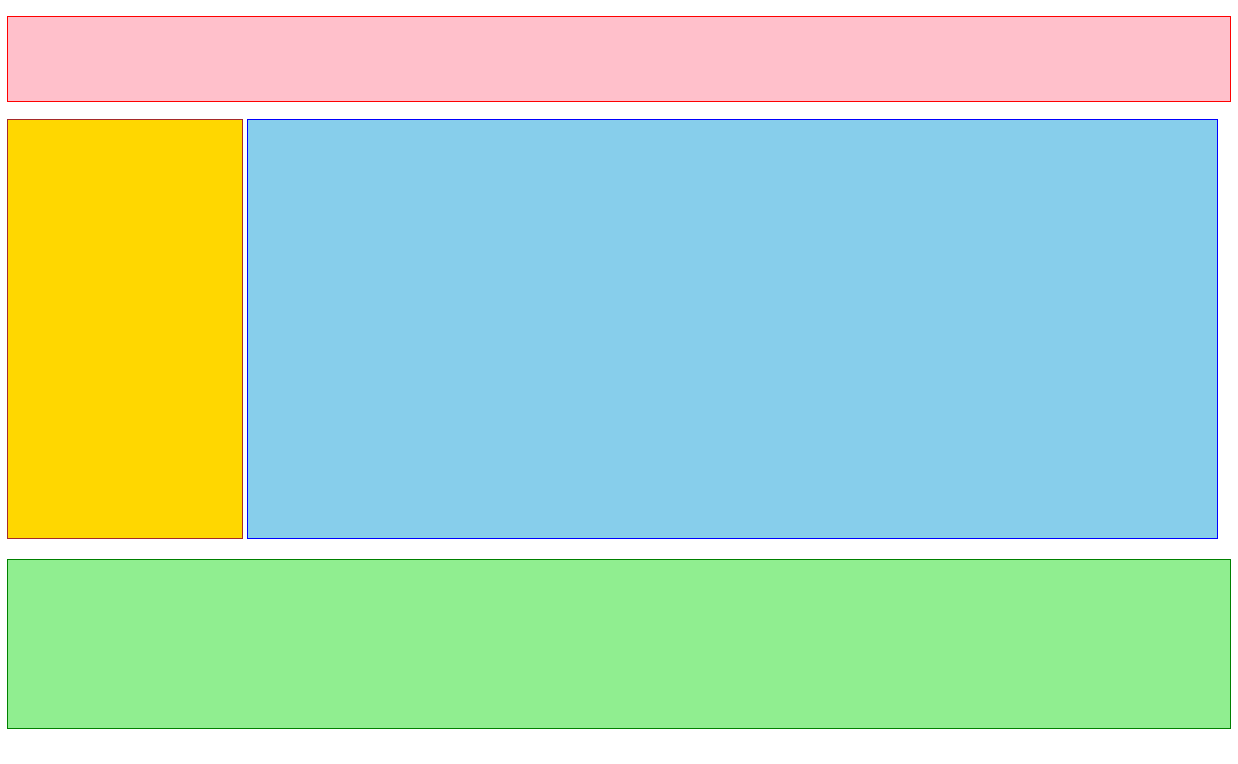
\includegraphics[width=\textwidth]{images/css-designing-html/exercise-responsive-2-wide.png}
        \caption{Wider than 800px}
        \label{fig:exercise-responsive-2-wide}
    \end{subfigure}
    \begin{subfigure}{.21\textwidth}\centering
        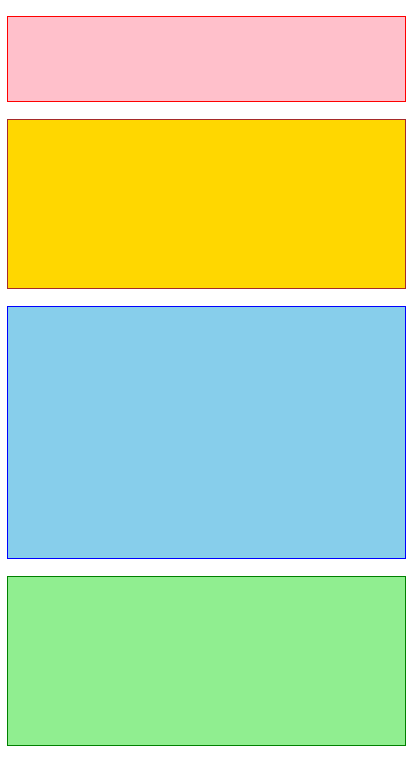
\includegraphics[width=\textwidth]{images/css-designing-html/exercise-responsive-2-small.png}
        \caption{Smaller than 800px}
        \label{fig:exercise-responsive-2-small}
    \end{subfigure}
    \caption{Webpage view of Exercise}
    \label{fig:exercise-responsive-2}
\end{figure}

\begin{codeenv}{code:exercise-responsive-web-2}{Exercise 5}\begin{verbatim}


<!doctype html>
<html>
<head>
    <title>CSS Exercise 5</title>
    <meta charset="utf-8">
    <meta name="viewport" content="width=device-width, initial-scale=1" >
    <link rel="stylesheet" text="type/css" href="./style.3.5.css">
</head>
<body>
    <div class="header"></div>
    <div class="body">
        <div class="navbar"></div>
        <div class="content"></div>
    </div>
    <div class="footer"></div>
</body>
</html>
\end{verbatim}
\end{codeenv}


    \chapter{Basics of Javascript}\label{ch:basics-of-javascript}
    \minitoc
    \section{Introducing Javascript} \label{sect:introducing-javascript}

자바스크립트(Javascript; JS)는 인터프리터형 프로그래밍 언어로, 웹 분야에서 광범위하게 사용되는 언어입니다. Front-end에서는 웹 페이지를 동적으로 작동하는 기능을 JS로 구현하며, 프론트엔드 프레임워크인 Angular.js, Vue.js 등에서도 널리 쓰입니다. 또한, front-end 뿐만 아니라 back-end 애플리케이션 역시 Node.js 엔진을 이용하여 JS로 구현할 수 있는 등, JS의 응용 범위는 광범위합니다. 이러한 JS의 성질로 인해, Stackoverflow에서 조사한 사용 빈도에 따른 컴퓨터 언어의 순위에서 7년째 1위를 차지하고 있습니다. 

\subsection*{컴파일형 언어와 인터프리터형 언어}

컴퓨터 언어는 그 언어로 작성된 프로그램의 실행 방식에 따라 컴파일러형 언어와 인터프리터형 언어, 두 가지로 나눌 수 있습니다. 컴파일러형 언어로 작성된 프로그램은 실행하기 위해 소스 코드를 기계어로 변환하는 과정, 즉 컴파일 과정이 필요합니다. C와 C++, Java, Rust, Go 등이 대표적인 컴파일러형 언어입니다. 

반면 인터프리터형 언어는 컴파일 과정 없이 인터프리터를 통해 소스 코드를 바로 실행할 수 있습니다. Python과 Javascript, Lisp 계열 언어들이 대표적인 인터프리터형 언어입니다. 컴파일 과정이 불필요하므로 인터프리터에 한 줄의 코드(정확히는 하나의 expression)를 입력한 후 바로 그 코드의 실행 결과를 확인할 수 있습니다. 

\begin{codeenv}{code:js-simple-example}{Simple Example of JS}\begin{verbatim}


> console.log('Hello World!');
undefined
Hello World!
> alert('Hello World!');
undefined
\end{verbatim}
\end{codeenv}

웹 브라우저의 개발자 도구에서 Console 탭을 열어 JS 코드를 한 줄씩 실행해볼 수 있습니다. \coderef{code:js-simple-example}을 실행해봅시다. \verb|console.log('Hello World!');|를 실행하면, 콘솔에 \verb|Hello World!|라는 문자열이 출력되는 것을 볼 수 있습니다. \verb|alert('Hello World!');|를 실행하면, 브라우저에 \verb|Hello World!| 문자열을 담은 경고창이 출력됩니다. 화면에 문자열을 출력하려면 \verb|console.log|를 사용해야 하지만, 콘솔에서 직접 JS 코드를 입력하여 실행하는 경우 코드 자체의 결과값도 출력됩니다. \verb|Hello World!| 외에 \verb|undefined|가 출력된 것은 이 때문입니다.

    \section{Declaration of Variables} \label{sect:declaration-of-variables}

\subsection*{ECMAScript}

ECMAScript는 스크립트 언어에 관한 규약으로, 줄여서 ES라고 하며, JS는 ES의 표준을 따른다. ES1이 1997년 출시된 이후 2015년 ES6가 출시되며 언어의 표준에 큰 변화가 발생하였고, 이후 지속적인 업데이트를 통해 2019년 ES9가 출시되어 현재\footnote{2021년}에 이르고 있다. 본 교재에서는 ES9을 표준으로 한 JS를 다룬다.

\subsection*{식별자의 선언}

JS는 다른 언어들과 마찬가지로 변수나 상수 등의 식별자(identifier)를 정의하고 사용할 수 있고, 모든 식별자에는 자료형이 있다. 다만 C나 Java 등과는 달리 식별자를 선언할 때 자료형을 명시해주지 않고, 인터프리터가 식별자에 할당되는 값을 분석하여 자료형을 스스로 지정한다.

변수, 상수, 함수 등은 camel case(예: \cd{parsedSourceInput}), 클래스는 pascal case(예: \cd{RequestHandler}), 상수는 대문자와 underscore(\cd{\_})로 작명(예: \cd{LENGTH\_LIMIT})한다. 또한, 숫자로 시작하지 않고 가급적 알파벳으로 시작하며, 식별자가 나타내는 바를 명확하게 알 수 있도록 작명한다.

식별자는 \cd{var}, \cd{let}, \cd{const} 등의 키워드를 이용하여 선언한다. 먼저, \cd{var}는 지금까지 널리 사용되어 온 키워드로, \cd{var}로 선언한 변수는 재선언할 수 있고, 값을 재할당할 수도 있다.

\begin{codeenv}{code:var-keyword}{Declaring Variable using \cd{var}}\begin{verbatim}
> var num1 = 3;
> num1;
3
> num1 + 5;
8
> num1 = 5;
5
> var num1 = 20;
\end{verbatim}
\end{codeenv}

반면 \cd{let}으로 선언한 변수는 값을 재할당할 수는 있으나, 재선언은 불가능하다.\footnote{Chrome의 개발자 도구를 이용하였을 때 재선언이 가능한 버그가 보고되었다. (2021년 기준)}

\begin{codeenv}{code:let-keyword}{Declaring Variable using \cd{let}}\begin{verbatim}
> let num2 = 3;
> num2 + 5;
8
> num2 = 5;
5
> let num2 = 20;
SyntaxError: redeclaration of let num2
\end{verbatim}
\end{codeenv}
\newpage

\cd{const}는 constant, 즉 상수(常數)의 약자로, \cd{const}로 선언한 상수는 재선언과 재할당이 모두 불가능하다.

\begin{codeenv}{code:const-keyword}{Declaring Constant using \cd{const}}\begin{verbatim}
> const constNum = 3;
undefined
> constNum + 5;
8
> constNum = 5;
TypeError: invalid assignment to const 'constNum'
> const constNum = 20;
Thrown:
SyntaxError: redeclaration of const constNum
\end{verbatim}
\end{codeenv}

\cd{var}는 JS 초창기부터 사용되어 왔던 식별자 선언 키워드인 반면, \cd{let}과 \cd{const}는 ES6 출시와 함께 추가된 식별자 선언 키워드이다. \cd{var}과 \cd{let}/\cd{const}는 재선언 가능성에서도 차이점이 있지만, 식별자에 접근할 수 있는 범위(scope)에도 차이가 있다.

\begin{codeenv}{code:var-let-scope}{Scope of var and let}\begin{verbatim}
> { var num1 = 1; }
> num1;
1
> { let num2 = 2; }
> num2;
Uncaught ReferenceError: num2 is not defined
\end{verbatim}
\end{codeenv}

\coderef{code:var-let-scope}\를 실행하면, \cd{var}로 선언된 \cd{num1}의 값은 정상적으로 출력되나, \cd{let}으로 선언된 \cd{num2}는 정의되지 않았다는 에러가 발생한다. 이렇듯 \cd{var}로 선언된 식별자는 선언된 블록 바깥에서 접근될 수 있고 함수 밖에서는 접근될 수 없는 function-scope이며, \cd{let}과 \cd{const}로 선언된 식별자는 선언된 블록 바깥에서 접근될 수 없는 block-scope이다.

\begin{tblenv}
    {tab:var-let-const-table}
    {Differences between \cd{var}, \cd{let} and \cd{const}}
    {>{\coll}m{0.08\tw}>{\coll}m{0.25\tw}>{\coll}m{0.25\tw}>{\coll}m{0.20\tw}}
    \thickhline
    키워드 & 재할당 (Reassignment) & 재선언 (Redeclaration) & 스코프 (Scope) \tabularnewline
    \hline
    \cd{var} & 가능 & 가능 & function-scope \tabularnewline
    \cd{let} & 가능 & 불가능 & block-scope \tabularnewline
    \cd{const} & 불가능 & 불가능 & block-scope \tabularnewline
    \thickhline
\end{tblenv}

ES6 이전에는 \cd{var}를 이용하여 변수를 선언하였으나, ES6 이후에는 \cd{let}과 \cd{const}가 재선언이 불가능하고, block-scope이기 때문에 \cd{var}의 사용은 지양되고 \cd{let}과 \cd{const}를 이용하여 변수와 상수를 선언하는 것이 권장된다. \cd{var}는 function-scope이기 때문에 코드의 네임스페이스를 오염\footnote{https://stackoverflow.com/questions/22903542/what-is-namespace-pollution}시키며, run-time에서 의도치 않은 논리적 오류를 발생시킬 수 있다. 반면 \cd{let}과 \cd{const}로 선언된 식별자는 block-scope이므로 네임스페이스 오염을 최소화할 수 있고, \cd{const}로 선언된 상수는 재할당이 불가능하므로 run-time에서 상수값이 변경되어 발생하는 논리적 오류를 방지할 수 있다.

    \section{Data Types} \label{sect:data-types}

JS에는 다음과 같은 7개의 자료형이 존재한다.

\begin{itemize}
    \item Primitive Types: number, string, boolean, undefined, null, symbol
    \item Compound Type: object
\end{itemize}

이번 절에서는 symbol형을 제외한 6가지 자료형과 배열을 다룬다.

\subsection*{Number}

number형은 수(數)를 저장하는 자료형으로, 정수, 유리수 등을 구별 없이 저장할 수 있고, 상호 연산이 가능하다.

\begin{codeenv}{code:number-type}{Number Type}\begin{verbatim}
> const num1 = 2;
> const num2 = 7.5;
> const num3 = 2 / 5;
> typeof num1;
'number'
> typeof num2;
'number'
> num1 * num2;
15
> num3;
0.4
\end{verbatim}
\end{codeenv}

number 자료형에는 일반적인 실수 이외에 \texttt{Infinity}와 \texttt{NaN}(not a number)이 있다. 두 값은 0으로 나누는 연산이 작용하면 발생한다.

\begin{codeenv}{code:infinity-nan}{Infinity and NaN}\begin{verbatim}
> 3 / 0;
Infinity
> typeof(3 / 0);
'number'
> 3 / (-0);
-Infinity
> 0 / 0;
NaN
> typeof(0 / 0);
'number'
\end{verbatim}
\end{codeenv}
\newpage

\subsection*{String}

string형은 문자열을 저장하는 자료형으로, string형 문자열 간에도 상호 계산이 가능하다.

\begin{codeenv}{code:string-type}{String Type}\begin{verbatim}
> const hello = 'Hello';
> const world = 'World';
> const helloWorld = hello + ' ' + world;
> helloWorld;
'Hello World'
> helloWorld.length;
11
> helloWorld[4];
'o'
> typeof helloWorld;
'string'
\end{verbatim}
\end{codeenv}

문자열을 표현할 때 큰따옴표(\texttt{"})나 작은따옴표(\texttt{'})를 사용하여 문자열을 감싸며, 서로 다른 문자로 감싸는 것은 불가능하다. 또한, 문자열 내에 감싸는 문자 등이 포함되어 있는 경우 역슬래시(\verb|\|)를 이용하여 escape 시켜야 한다.

\begin{codeenv}{code:string-type-assign}{Assigning Value on String Type Variable}\begin{verbatim}
> "String";
'String'
> 'String';
'String'
> "String';
Uncaught SyntaxError: Invalid or unexpected token
> "McDonald's";
'McDonald\'s'
> console.log("McDonald's");
McDonald's
\end{verbatim}
\end{codeenv}

\subsection*{Boolean}

boolean형은 논리적인 요소를 나타내며, \texttt{true}와 \texttt{false} 두 가지의 값이 가능하다.

\begin{codeenv}{code:boolean-type}{Boolean Type}\begin{verbatim}
> 1 == 1;
true
> 1 > 3;
false
> true == false;
false
> true != false;
true
> const isNumberEven = (5 % 2 == 0);
> isNumberEven;
false
\end{verbatim}
\end{codeenv}

\subsection*{Object}

object형, 즉 객체형이란 key와 value를 가질 수 있는 자료형이다. 예를 들어, 어떠한 학생에 대한 정보를 다룰 때, 학생의 학번, 이름, 학과, 재학 여부 등을 서로 다른 변수에 저장하지 않고, \texttt{student}라는 객체형 식별자에 저장하여 일괄적으로 다룰 수 있다. Key는 같은 계층에서 유일한 문자열이고, value에는 숫자, 문자열 등 자료형에 상관없이 모든 종류의 식별자가 가능하다. 즉, 객체 내부에 또 다른 객체가 포함될 수 있어, 계층이 있는 데이터(hierarchial data)를 형성하는 것이 가능하다.

\begin{codeenv}{code:object-type}{Object Type}\begin{verbatim}
> const person = {
    age: 21,
    name: 'Frank',
    height: 170,
    isMale: true,
};
> person;
{ age: 21, name: 'Frank', height: 170, isMale: true }
> person.age;
21
> person['age'];
21
> !person.isMale;
false
> person.weight = 60;
60
> person;
{ age: 21, name: 'Frank', height: 171, isMale: true, weight: 60 }
\end{verbatim}
\end{codeenv}

\subsection*{Undefined and Null}

undefined형과 null형은 각각 값이 할당되지 않은 식별자와 값을 모르는 식별자가 갖는 자료형이며, 두 자료형의 값은 각각 항상 \texttt{undefined}와 \texttt{null}이다.

\begin{codeenv}{code:undefined-type}{Undefined Type}\begin{verbatim}
> let undefVar;
> undefVar;
undefined
> typeof undefVar;
'undefined'
\end{verbatim}
\end{codeenv}

JS에는 null 자료형 식별자를 \texttt{typeof} 함수를 이용하여 확인할 때 잘못된 자료형을 반환받는 버그를 가지고 있다. 이는 매우 오래된 버그이므로 고치는 것이 불가능하다고 하며, 변수가 \texttt{null}임을 확인하기 위해서는 값을 직접 비교하여야 한다.
\newpage

\begin{codeenv}{code:null-type}{Null Type}\begin{verbatim}
> const nullVar = null;
> typeof null;
'object'
> nullVar == null;
true
\end{verbatim}
\end{codeenv}

\subsection*{Array}

배열은 index를 가지는, 복수의 자료를 저장할 수 있는 자료구조이다. JS에서는 각 원소의 자료형에 제한이 없어 서로 다른 자료형의 원소를 하나의 배열에 저장할 수 있으며, 배열의 크기가 정해져 있지 않어 각종 메서드(method)를 이용하여 원소를 자유롭게 넣고 뺄 수 있다.

\begin{codeenv}{code:js-array}{Array}\begin{verbatim}
> const arr = [0, 1, 1.5, true, 'hungry'];
> arr.length;
5
> arr[3];
true
> arr[4];
'hungry'
> arr.push('new element');
6
> arr;
[ 0, 1, 1.5, true, 'hungry', 'new element' ]
\end{verbatim}
\end{codeenv}

    \section{Statements and Functions} \label{sect:statements-and-functions}

\subsection*{Comparison}

JS의 비교 연산은 여타 언어들과 유사하게 \texttt{==}과 \texttt{!=} 연산자로 수행될 수 있으며, 비교 연산의 결과가 참이면 \texttt{true}, 거짓이면 \texttt{false}를 반환한다. 그러나 JS에서는 \texttt{==}이나 \texttt{!=} 연산자로 비교 연산을 수행하였을 때 문제가 발생할 수 있다.

\begin{codeenv}{code:loose-equality}{Loose Equality}\begin{verbatim}


> 0 == 0;
true
> 0 == '0';
true
\end{verbatim}
\end{codeenv}

\coderef{code:loose-equality}에서는 number형의 \texttt{0}과 string형의 \texttt{'0'}을 비교하였다. 두 값은 자료형이 다름에도 불구하고 같다는 결과가 도출되는데, 그 이유는 JS에서 \texttt{==}과 \texttt{!=} 연산자를 이용하여 비교 연산을 수행할 때, 두 값에 대해 자의적으로 자료형 변환(type coercion)을 수행한 뒤 변환된 값을 비교하기 때문이다. 이렇게 비교 연산에서 \texttt{==}과 \texttt{!=} 연산자를 사용하여 자료형 변환이 이루어진 뒤 수행되는 연산을 loose equality이라고 한다. JS가 수행하는 타입 변환 규칙은 복잡하기 때문에 loose equality는 사용하지 않는 것이 권장된다.

\begin{figure}[htb]\vspace{10pt}\centering
    \begin{subfigure}{.231\textwidth}\centering
        
\includegraphics[width=\textwidth]{images/basics-of-javascript/loose-equality-syllogism.png}
        \caption{Syllogism does not hold}
        \label{fig:loose-equality-syllogism}
    \end{subfigure}
    \begin{subfigure}{.729\textwidth}\centering
        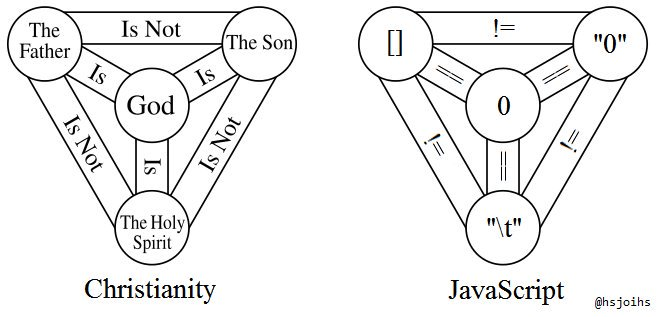
\includegraphics[width=\textwidth]{images/basics-of-javascript/loose-equality-trinity.jpg}
        \caption{The Javascript Trinity of \texttt{0}}
        \label{fig:loose-equality-trinity}
    \end{subfigure}
    \caption{Loose Equality Memes}
    \label{fig:loose-equality-memes}
\end{figure}

이러한 이유로 JS에서는 loose equality 대신 자료형까지 고려하여 값을 비교하는 strict equality가 권장된다. Strict equality는 \texttt{===}과 \texttt{!==} 연산자를 이용하여 수행될 수 있다.

\begin{codeenv}{code:strict-equality}{Strict Equality}\begin{verbatim}


> 0 === 0;
true
> 0 === '0';
false
\end{verbatim}
\end{codeenv}

\figref{fig:comparison-table}는 loose equality와 strict equality의 결과를 정리한 표이다. 이 결과를 알아두어서 나쁠 것은 없지만, 가독성이 좋고 논리적 오류를 최소화할 수 있는 strict equality를 사용하는 것이 훨씬 효율적이다.

\begin{figure}[htb]\vspace{10pt}\centering
    \begin{subfigure}{.45\textwidth}\centering
        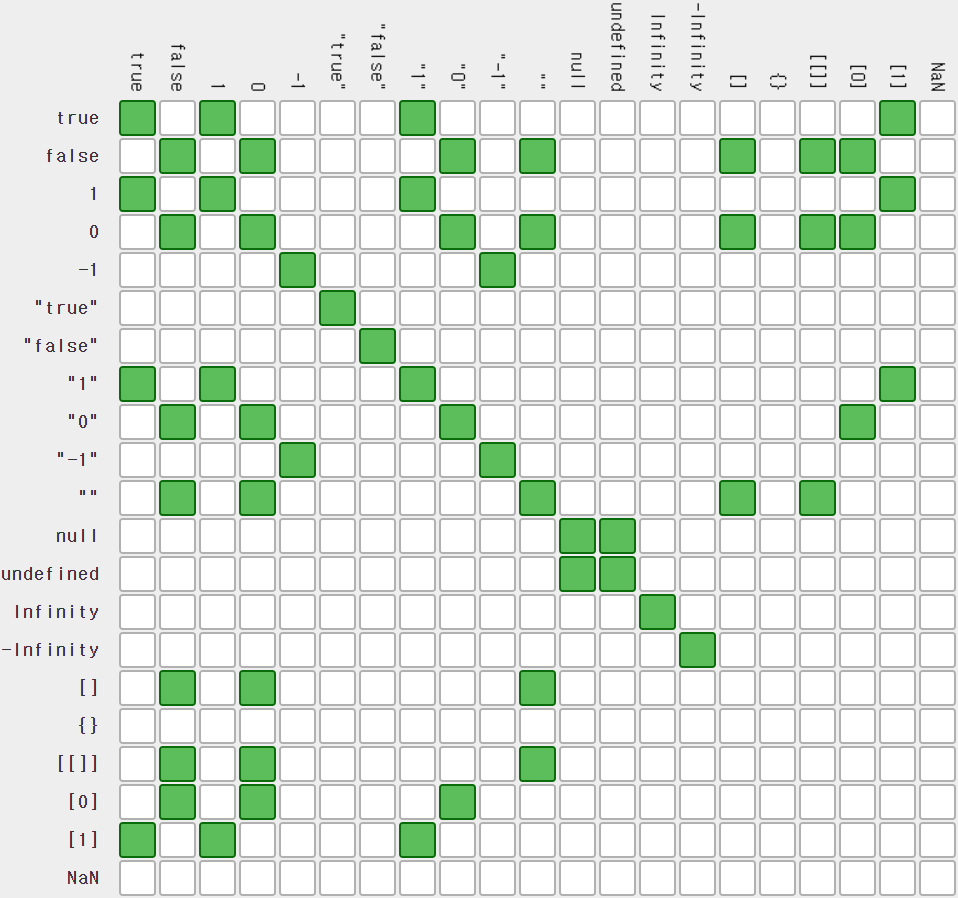
\includegraphics[width=\textwidth]{images/basics-of-javascript/loose-equality.png}
        \caption{Loose Equality}
        \label{fig:loose-equality-table}
    \end{subfigure}
    \begin{subfigure}{.45\textwidth}\centering
        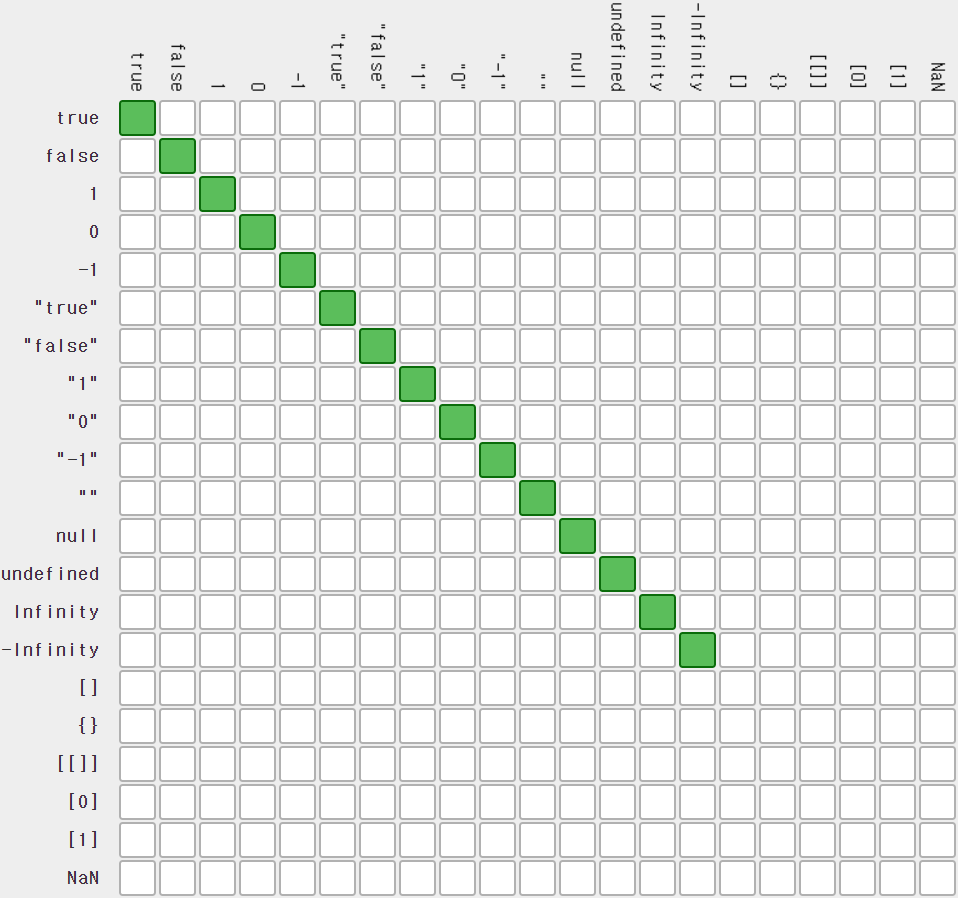
\includegraphics[width=\textwidth]{images/basics-of-javascript/strict-equality.png}
        \caption{Strict Equality}
        \label{fig:strict-equality-table}
    \end{subfigure}
    \caption{Equality table of JS. Colored cell implies \texttt{true}}
    \label{fig:comparison-table}
\end{figure}

% Image from https://dorey.github.io/JavaScript-Equality-Table/

\subsection*{Conditional Statements}

JS의 조건문은 여타 언어들의 조건문과 유사하게 \texttt{if}, \texttt{if else}, \texttt{else}의 키워드를 사용한다.

\begin{codeenv}{code:if-else-stmt}{If-else Statement}\begin{verbatim}


> const num = 100;
> if (num % 2 === 0) {
      console.log('num is even');
  } else {
      console.log('num is odd');
  }
num is even
> const isEven = num % 2 === 0;
> if (isEven) {
      console.log('num is even');
  } else {
      console.log('num is odd');
  }
num is even
> const remainder = num % 3;
> if (remainder === 0) {
      console.log('remainder is 0');
  } else if (remainder === 1) {
      console.log('remainder is 1');
  } else {
      console.log('remainder is 2');
  }
remainder is 1
\end{verbatim}
\end{codeenv}
\pagebreak

또한, switch-case문과 삼항 연산자 \texttt{? :}도 지원한다.

\begin{codeenv}{code:switch-case-stmt-tertiary}{switch-case Statement and Tertiary operator}\begin{verbatim}


> const num = 100;
> const remainder = num % 3;
> switch (remainder) {
      case 1:
          console.log('remainder is 1'); break;
      case 2:
          console.log('remainder is 2'); break;
      default:
          console.log('remainder is 0');
  }
remainder is 1
> const quotient = ((num % 7 === 0) ? num : (num - num % 7)) / 7;
14
\end{verbatim}
\end{codeenv}

\subsection*{Iteration Statements}

JS의 반복문 역시 여타 언어들과 유사하게 \texttt{for}문을 사용한다.

\begin{codeenv}{code:for-stmt}{반복문}\begin{verbatim}


> const fruits = ['apple', 'orange', 'mango', 'grapes'];
> for (let i = 0; i < fruits.length; i++) {
      console.log(fruits[i]);
  }
apple
orange
mango
grapes
\end{verbatim}
\end{codeenv}

\coderef{code:for-stmt}와 같이 반복문을 사용할 때마다 배열의 index를 어떠한 변수에 저장하고, 이를 이용해 배열의 각 원소를 가져오는 것은 번거롭다. for-of문을 사용하여 반복문을 간결하게 사용할 수 있다.

\begin{codeenv}{code:for-of-stmt}{for-of문}\begin{verbatim}


> const fruits = ['apple', 'orange', 'mango', 'grapes'];
> for (const fruit of fruits) {
    console.log(fruit);
}
apple
orange
mango
grapes
\end{verbatim}
\end{codeenv}

\coderef{code:for-of-stmt}과 같이 for-of문은 배열의 각 원소를 차례대로 특정 변수(\texttt{fruit})에 저장하고, for문 내에서 사용할 수 있도록 한다. 이렇게 for-of문을 사용하면 각 원소의 index는 알 수 없지만, 개별 원소는 직접 가져와 반복문을 간결하게 작성할 수 있는 장점이 있다.

\begin{codeenv}{code:for-in-stmt}{for-in문}\begin{verbatim}


> const person = { age: 21, name: 'Frank', height: 171, isMale: true, weight: 60 };
> for (const key in person) {
      console.log(key + ': ' + person[key]);
  }
age: 21
name: Frank
height: 171
isMale: true
weight: 60
\end{verbatim}
\end{codeenv}

for-of문과 유사하여 헷갈리기 쉬운 for-in문은 객체(object)에 대해 동작하며, for-in문 내부에서 객체의 각 key를 직접 가져와 사용할 수 있고, 이를 이용해 value에도 바로 접근할 수 있다.

\subsection*{Functions}

\begin{codeenv}{code:basic-function}{Function Declaration and Call}\begin{verbatim}


> function add(x, y) {
      return x + y;
  }
> add(1, 2);
3
> add('1', '2');
'12'
\end{verbatim}
\end{codeenv}

JS에서 함수는 \coderef{code:basic-function}와 같이 \texttt{function} 키워드를 이용하여 함수의 이름과 인자를 작성하고, 중괄호 내부에 함수 내용을 작성한다. JS에서는 식별자의 자료형을 따로 지정하지 않으므로 인자와 반환값의 자료형 역시 따로 지정하지 않는다는 점을 주목하여야 한다. 따라서, \coderef{code:basic-function}의 함수는 마지막 줄과 같이 사용될 수도 있다.

\begin{codeenv}{code:arrow-function}{Arrow Function}\begin{verbatim}


> const add = (x, y) => {
      return x + y;
  };
> add(1, 2);
3
> const square = num => num * num;
> square(5);
25
\end{verbatim}
\end{codeenv}

ES6 이후에는 \coderef{code:arrow-function}과 같이 arrow(\texttt{=>})를 사용하여 함수를 비교적 간결하게 정의하는 것이 권장된다. 표현식을 관찰해보면, \texttt{x}와 \texttt{y} 두 인자를 받아 덧셈을 수행한 뒤 반환하는 함수를 \texttt{add}라는 식별자에 할당하였다. JS에서는 함수 역시 하나의 변수 또는 상수로 취급될 수 있어 arrow function을 이용하여 함수를 작성할 수 있고, 함수를 다른 함수의 인자로 넘길 수도 있다.

Arrow function의 인자가 1개일 때는 인자 부분의 괄호를 생략할 수 있고, 함수에 값을 반환하는 부분만 있는 경우 중괄호와 \texttt{return} 키워드가 생략될 수 있다.

\begin{codeenv}{code:anonymous-function}{Anonymous Function}\begin{verbatim}


> num => num * num;
function (num)
> ((base, power) => {
      res = 1;
      for (let i = 0; i < power; i++) res *= base;
      return res;
  })(3, 5);
243
\end{verbatim}
\end{codeenv}

Arrow function을 활용하면 \coderef{code:anonymous-function}와 같이 익명 함수(anonymous function)를 선언할 수 있다.

\begin{codeenv}{code:high-order-function}{Anonymous Function with High-order Function}\begin{verbatim}


> const arr = ['a', 'bb', 'ccc', 'dddd'];
> const lengths = arr.map(e => e.length);
> lengths;
[ 1, 2, 3, 4 ]
\end{verbatim}
\end{codeenv}

함수 중에는 함수를 인자로 쓰는 함수가 있는데, 이러한 함수를 고차원 함수(high-order function)라고 한다. 익명 함수는 재사용하지 않는 함수를 고차원 함수의 인자로 넘길 때 유용하게 사용된다. \coderef{code:high-order-function}에서 \texttt{map} 함수는 배열의 각 원소를 인자로 받은 함수의 인자로 주어 실행한 결과를 배열로 반환한다. JS에서는 이러한 고차원 함수가 특히 많으므로 고차원 함수를 사용하면서 익명 함수를 빈번하게 사용하게 될 것이다.

\begin{codeenv}{code:foreach-method}{\texttt{forEach} Method}\begin{verbatim}


> const fruits = ['apple', 'orange', 'mango', 'grapes'];
> fruits.forEach(fruit => console.log(fruit));
apple
orange
mango
grapes
> const printFruit = (fruit, idx) => console.log('#' + (idx + 1) + ': ' + fruit);
> fruits.forEach(printFruit);
#1: apple
#2: orange
#3: mango
#4: grapes
\end{verbatim}
\end{codeenv}

익명 함수를 이용하여, 앞에서 다룬 for-of 문을 \coderef{code:foreach-method}과 같이 \texttt{forEach} 함수를 사용하여 바꿀 수 있다. \texttt{forEach} 함수는 각 원소뿐만 아니라 원소의 index와 원본 배열까지도 받아 사용할 수 있다.

    \section{Built-in Objects} \label{sect:built-in-objects}

\sectref{sect:data-types}에서 객체에 대해 다룬 바 있는데, 이번 절에서는 객체에 대해 더 자세히 알아보자. JS에서 number형이나 string형의 식별자, 배열, 함수 등은 모두 객체\footnote{object형은 아니다.}이고, 그러므로 객체라는 개념을 정확히 이해하기 위해 객체 지향형 프로그래밍(Object-Oriented Programming)을 공부해야 하지만, 본 교재에서 다루는 내용과는 다소 거리가 있으므로 이번 절에서는 클래스와 메서드 등의 기초 개념만 다룬다. 또한, JS에서 기본적으로 제공되는 객체(built-in objects)의 종류와 속성과 메서드 등의 사용 방법에 대해 학습한다.

\subsection*{Property와 Method}

\coderef{code:object-type}(\pageref{code:object-type}쪽)에서 \texttt{person}이라는 객체에 \texttt{age}, \texttt{name}, \texttt{height}, \texttt{isMale}의 네 속성과 그 값을 부여하였다. 이때 \texttt{person} 객체의 속성의 값을 이용하여 수행하는 작업을 생각해보자. 예를 들어 새해가 되어 \texttt{age} 값을 증가시켜주는 작업은 \texttt{age}의 값을 \texttt{1}만큼 증가시키는 작업이다. 이 작업은 매우 간단하지만, 복잡하고 긴 과정을 거쳐야 하는 작업일 수도 있으므로 \texttt{increaseAge}라는 함수를 만들어두고 사용하는 것이 훨씬 효율적일 것이다.

그런데 JS 파일에 함수를 만들어두고 사용하면 어떤 부작용이 있겠는가? 객체가 많은 프로그램의 경우는 함수의 수가 지나치게 많아져 가독성이 저하되고, 개발자가 헷갈리기 쉬워지고 코드 분석도 어려워지는 등 효율성이 저하될 수 있다. 또한, 다른 객체에 대해 유사한 작업을 수행하는 함수가 있다면 함수 이름이 겹쳐 namespace 오염이 일어날 수 있고, 함수 이름을 비효율적으로 짓게 된다. 따라서 객체의 속성값을 이용하는 함수는 객체 내부에 정의하여 namespace 오염과 부작용을 방지하고, 이를 메서드(method)라고 한다.

\begin{codeenv}{code:object-method}{Method of Object}\begin{verbatim}


> const person = {
      age: 21,
      name: 'Frank',
      height: 170,
      isMale: true,
      increaseAge: function () { this.age++ },
  };
> person.increaseAge();
> person.age;
22
\end{verbatim}
\end{codeenv}

메서드는 \coderef{code:object-method}과 같이 key에 메서드 이름을 작성하고 value에 메서드가 수행할 작업을 함수의 형태로 할당한다. 앞의 \texttt{increaseAge} 메서드는 자신이 속한 \texttt{person} 객체의 \texttt{age} 값을 \texttt{1}만큼 증가시켜야 하는데, 함수 내에 \texttt{age}가 선언되어 있지 않아 직접 접근할 수 없다. 이때 \texttt{this} 키워드를 사용하면 자기 자신이 속한 객체에 접근할 수 있다.\footnote{\texttt{this}는 자기 자신의 객체 외에도 다른 종류의 객체를 가리킬 수도 있다.} 즉 \texttt{increaseAge} 메서드 내부의 \texttt{this}는 \texttt{person}을 가리키고, \texttt{increaseAge}는 자신의 속성 \texttt{age}의 값을 \texttt{1}만큼 증가시킨다.

\begin{codeenv}{code:object-simple-method}{Simple Method Syntax}\begin{verbatim}


> const person = {
      age: 21,
      increaseAge() { this.age++ },
  };
> person.increaseAge();
> person.age;
22
\end{verbatim}
\end{codeenv}

ES6의 축약 메서드 표현법에 따라 \coderef{code:object-simple-method}과 같이 축약하여 표현할 수 있다.

메서드를 표현할 때 arrow function을 이용하면 오류가 발생할 여지가 크다는 점을 주의해야 한다. 화살표 함수는 \texttt{this}가 가리키는 객체를 정하는 방식이 일반적인 함수와 다르므로\footnote{https://poiemaweb.com/es6-arrow-function} 메서드를 표현할 때는 arrow function보다는 일반적인 함수 표현 방식을 사용하는 것이 좋다.

\subsection*{Class and Instance}

앞에서는 Frank라는 이름을 가진 사람에 대한 정보를 다루기 위해 \texttt{person}이라는 객체를 생성하고 속성과 메서드를 정의하였다. 그런데 Frank라는 사람 한 명뿐만 아니라 같은 속성을 갖는 수많은 사람에 대한 정보를 다루려고 할 때 \coderef{code:object-method}과 같이 객체를 일일이 생성하는 방식은 매우 비효율적이며 재사용성이 크게 떨어진다.

이렇게 동일한 형태의 객체들을 생성하기 위해 클래스(class)를 이용하여 객체들의 구조를 표현하며, 클래스는 설계도와 같은 역할을 한다. 클래스는 각 객체가 갖는 속성, 상수, 메서드 등에 대한 정보의 집합이다. 그리고 이러한 설계도, 즉 클래스에 따라 생성된 각 객체를 인스턴스(instance)라고 한다. 예를 들어 \texttt{Person}이라는 클래스가 있다면 이 클래스에 따라 생성된 객체 \texttt{frank}, \texttt{david}, \texttt{jennie} 등은 인스턴스이다.

인스턴스를 생성하려면 클래스라는 설계도를 이용하여 객체를 생성하는 매개체가 필요하다. 이 매개체를 생성자(constructor)라고 부르며, 생성자는 인스턴스를 생성할 때 필요한 정보를 받아, 설계도에 따라 객체의 속성이나 메서드를 정한다. 예를 들어, 앞의 \texttt{Person} 클래스의 생성자는 나이, 이름, 키, 성별 등의 정보를 받아 \texttt{age}, \texttt{name}, \texttt{height}, \texttt{isMale}의 속성값에 저장할 것이다. 또한, 생성자는 여러 유의미한 정보가 응집되어 있는 정보를 나누어 서로 다른 속성에 저장하기도 한다. 예를 들어, 학생의 학번을 받아서 입학 연도, 소속 학과, 개인 일련번호 등의 정보를 저장하는 \texttt{Student}라는 클래스를 가정한다면 이 클래스의 생성자는 학번을 분석하여 \texttt{admissionYear}, \texttt{department}, \texttt{serialNumber} 등의 속성에 분석한 값들을 저장할 수 있다.

속성이나 메서드는 자신이 속한 클래스와 연관성은 크지만, 생성자가 필요하지 않을 수도 있다. 이러한 메서드를 정적(static) 속성 및 정적 메서드라고 하며, 생성자를 사용하지 않고 클래스에서 직접 속성이나 메서드를 호출할 수 있다.
\newpage

\subsection*{Global Methods(Functions)}

다음 메서드들은 객체를 명시하지 않고 함수 형태로 사용할 수 있는 메서드들이다. 이 함수들은 사실 전역 객체(global object)의 메서드이므로 함수처럼 사용할 수 있는 것이다.

\begin{itemize}
    \item \texttt{isFinite(testValue) => boolean}: 주어진 값이 유한한지 판별하는 메서드; \texttt{testValue}를 인자로 받아 \texttt{Infinity}, \texttt{NaN}, \texttt{undefined}이면 \texttt{false}, 아니면 \texttt{true}를 반환한다.
    \item \texttt{isNaN(testValue) => boolean}: 주어진 값이 \texttt{NaN}인지 판별하는 메서드; \texttt{testValue}를 인자로 받아 \texttt{NaN}이면 \texttt{false}, 아니면 \texttt{true}를 반환한다.
    \item \texttt{parseInt(string[, radix]) => number}: 주어진 문자열을 숫자로 변환하는 메서드; \texttt{string}과 \texttt{radix}를 인자로 받아, \texttt{string}을 \texttt{radix}진법의 정수로 변환하여 반환한다. 주어진 값을 정수로 변환할 수 없다면 \texttt{NaN}을 반환하며, \texttt{radix}가 주어지지 않을 때는 \texttt{string}이 \texttt{0x}나 \texttt{0X}로 시작하면 16진수로, 그 외에는 10진수로 변환한다.
\end{itemize}

\begin{codeenv}{code:global-methods}{Global Methods}\begin{verbatim}


> isFinite(3/0);
false
> isNaN(0/0);
true
> parseInt('3.5');
3
> parseInt('hello');
NaN
\end{verbatim}
\end{codeenv}

\subsection*{String Objects}

string형 식별자, 즉 \texttt{String} 객체의 자주 쓰이는 속성이나 메서드이며, MDN 문서\footnote{https://developer.mozilla.org/en-US/docs/Web/JavaScript/Reference/Global\_Objects/String}에서 더 자세하게 확인할 수 있다.

\begin{itemize}
    \item \texttt{length}: 문자열의 길이를 값으로 갖는 속성
    \item \texttt{includes(searchString[, position]) => boolean}: 문자열에 주어진 문자열이 포함되는지 판별하는 메서드; 원래 문자열에 \texttt{searchString} 문자열이 \texttt{position}번째 문자 이후에 포함되면 \texttt{true}, 포함되지 않으면 \texttt{false}를 반환한다. \texttt{position}의 기본값은 \texttt{0}이다.
    \item \texttt{replace(substr, newSubstr) => string}: 문자열의 일부분을 다른 문자열로 대치(代置)하여 반환하는 메서드; 원래 문자열에서 처음으로 나오는 \texttt{substr} 문자열 부분을 \texttt{newSubstr}로 대치한다. \texttt{substr}은 정규식 형태로 주어질 수도 있다.
    \item \texttt{replaceAll(substr, newSubstr) => string}: 문자열의 일부분을 모두 다른 문자열로 대치하여 반환하는 메서드; \texttt{replace} 메서드와 유사하게 동작하나 \texttt{substr} 문자열 부분을 모두 \texttt{newSubstr}로 대치한다.
    \item \texttt{split([separator, limit]) => Array<string>}: 문자열을 주어진 문자열을 기준으로 분리하여 문자열의 배열로 반환하는 메서드; 원래 문자열에서 \texttt{separator}를 기준으로 분리하여 최대 \texttt{limit}개의 문자열을 반환한다. \texttt{separator}가 주어지지 않으면 분리되지 않으며, \texttt{limit}이 주어지지 않으면 반환하는 문자열 배열의 길이에 제한이 없다.
    \item \texttt{substring(indexStart[, indexEnd]) => string}: 문자열의 일부분을 추출하는 메서드; \texttt{indexStart}번째 문자부터 \texttt{indexEnd}번째 문자 직전까지의 문자열을 추출하여 반환하며, \texttt{indexEnd}의 기본값은 \texttt{length} 속성값이다.
    \item \texttt{toLowerCase() => string}: 문자열 중 알파벳을 모두 소문자로 바꾸어 반환하는 메서드
    \item \texttt{toUpperCase() => string}: 문자열 중 알파벳을 모두 대문자로 바꾸어 반환하는 메서드
    \item \texttt{trim() => string}: 문자열의 앞뒤 whitespace를 모두 제거하여 반환하는 메서드
\end{itemize}

\begin{codeenv}{code:string-methods}{String Object Methods}\begin{verbatim}


> const str = '  Hello World!\t';
> str.length;
15
> str.includes('ll');
true
> str.replace('World', 'Korea');
'  Hello Korea!\t'
> str.split('o');
[ '  Hell', ' W', 'rld!\t' ]
> str.substring(6);
'o World!\t'
> str.toUpperCase();
'  HELLO WORLD!\t'
> str.trim();
'Hello World!'
\end{verbatim}
\end{codeenv}

\subsection*{Array Objects}

배열에서 자주 쓰이는 속성이나 메서드이며, MDN 문서\footnote{https://developer.mozilla.org/en-US/docs/Web/JavaScript/Reference/Global\_Objects/Array}에서 더 자세하게 확인할 수 있다. 많은 메서드가 high-order 함수임을 확인할 수 있다.

\begin{itemize}
    \item \texttt{length}: 배열의 길이를 값으로 갖는 속성
    \item \texttt{concat([arr1, arr2, ..., arrN]) => Array}: 원래 배열의 뒤에 여러 배열을 이어붙여 반환하는 메서드
    \item \texttt{filter(fn(element[, index, array]) => boolean) => Array}: 배열의 원소 중 주어진 test를 통과한 원소들의 배열을 반환하는 메서드. 배열의 원소 중 \texttt{fn}의 반환값이 \texttt{true}인 원소들의 배열을 반환한다. \texttt{fn}은 원소의 값, index, 원본 배열을 인자로 받아 boolean 값을 반환한다.
    \item \texttt{find(fn(element[, index, array]) => boolean) => Any}: 배열의 원소 중 주어진 함수를 만족하는 첫 번째 원소를 반환하는 메서드
    \item \texttt{findIndex(fn(element[, index, array]) => boolean) => number}: 배열의 원소 중 주어진 함수를 만족하는 첫 번째 원소의 index를 반환하는 메서드
    \item \texttt{forEach(fn(element[, index, array]))}: 배열의 각 원소에 대해 주어진 함수를 실행하는 메서드
    \item \texttt{includes(searchElement[, fromIndex]) => boolean}: 배열의 원소에 주어진 원소가 있는지 판별하는 메서드; 배열의 \texttt{fromIndex}번째 원소 이후에 \texttt{searchElement}가 있으면 \texttt{true}를 반환한다. \texttt{fromIndex}의 기본값은 \texttt{0}이다.
    \item \texttt{join([separator]) => string}: 배열의 모든 원소를 주어진 문자열로 이어붙인 문자열을 반환하는 메서드
    \item \texttt{map(fn(element[, index, array]) => Any) => Array}: 배열의 각 원소에 대한 주어진 함수의 반환값의 배열을 반환하는 메서드
    \item \texttt{pop() => Any}: 배열의 마지막 원소를 제거하고, 마지막 원소의 값을 반환하는 메서드
    \item \texttt{push([val0, val1, ..., valN]) => number}: 배열의 끝에 주어진 값을 배열의 원소로 차례대로 삽입하고, 값이 모두 삽입된 배열의 길이를 반환하는 메서드
    \item \texttt{reverse() => Array}: 배열의 원소들의 순서를 반대로 뒤집어 반환하는 메서드; 원본 배열도 뒤집힌다는 점을 주의하여야 한다.
    \item \texttt{slice([start, end]) => Array}: 배열의 일부분을 추출하는 메서드; \texttt{start}번째 원소부터 \texttt{end}번째 원소 직전까지의 원소를 반환하며, \texttt{start}의 기본값은 \texttt{0}, \texttt{end}의 기본값은 \texttt{length} 속성이다.
    \item \texttt{sort([compareFn(firstEl, secondEl) => number])}: 배열의 원소들을 주어진 함수에 따라 정렬하여 반환하는 메서드; \texttt{compareFn}은 두 비교 대상 원소를 인자로 받으며, 반환값이 음수인 경우 \texttt{firstEl}이, 양수인 경우 \texttt{secondEl}이 앞에 정렬된다. \texttt{compareFn}이 주어지지 않은 경우 알파벳 순서대로 정렬된다. 원본 배열도 정렬된다는 점을 주의하여야 한다.
\end{itemize}

\begin{codeenv}{code:array-methods}{Array Methods}\begin{verbatim}


> const arr = ['apple', 'orange', 'banana'];
> arr.length;
3
> arr.concat(['cherry', 'grapes']);
[ 'apple', 'orange', 'banana', 'cherry', 'grapes' ]
> arr.filter(fruit => fruit.length === 6);
[ 'orange', 'banana' ]
> arr.findIndex(fruit => fruit[0] === 'b');
2
> arr.includes('lemon');
false
> arr.join(' + ');
'apple + orange + banana'
> arr.map((elmt, index) => '#' + index + ': ' + elmt);
[ '#0: apple', '#1: orange', '#2: banana' ]
> arr.pop();
'banana'
> arr.push('cherry', 'grapes');
4
> arr.reverse();
[ 'grapes', 'cherry', 'orange', 'apple' ]
> arr.sort();
[ 'apple', 'cherry', 'grapes', 'orange' ]
> arr.sort((first, second) => {
      const firstLength = first.split('e')[0].length;
      const secondLength = second.split('e')[0].length;
      return firstLength - secondLength;
  });
[ 'cherry', 'apple', 'grapes', 'orange' ]
\end{verbatim}
\end{codeenv}
\newpage

\subsection*{Date Objects}

\texttt{Date} 클래스는 날짜와 시간을 다루는 클래스이며, \texttt{Date} 클래스의 인스턴스를 생성하기 위해서는 생성자를 이용하여야 하며, \texttt{Date} 클래스의 생성자는 네 가지가 있다.

\begin{itemize}
    \item \texttt{new Date()}: 현재 날짜/시각을 나타내는 \texttt{Date} 객체를 생성한다.
    \item \texttt{new Date(msec)}: Epoch 시각\footnote{1970년 1월 1일 자정 UTC}으로부터 \texttt{msec}밀리초가 지난 후의 날짜/시각을 나타내는 \texttt{Date} 객체를 생성한다.
    \item \texttt{new Date(dateStr)}: \texttt{dateStr}을 분석하여 문자열이 표현하는 날짜/시각을 나타내는 \texttt{Date} 객체를 생성한다.
    \item \texttt{new Date(year, mon[, day, hrs, min, sec, msec])}: \texttt{year}년 \texttt{mon}월 \texttt{day}일 \texttt{hrs}시 \texttt{min}분 \texttt{sec}초 \texttt{msec} 밀리초에 해당하는 날짜/시각을 나타내는 \texttt{Date} 객체를 생성한다. \texttt{mon}의 값은 \texttt{0}이 1월, \texttt{11}이 12월이다.
\end{itemize}

\texttt{Date} 객체의 메서드 몇 가지를 나열하면 다음과 같으며, MDN 문서\footnote{https://developer.mozilla.org/en-US/docs/Web/JavaScript/Reference/Global\_Objects/Date}에서 더 자세하게 확인할 수 있다.

\begin{itemize}
    \item \texttt{now() => number}: Epoch 시각으로부터 현재까지 흐른 시간을 밀리초 단위로 반환하는 정적 메서드
    \item \texttt{getFullYear() => number}: \texttt{Date} 객체의 날짜/시각의 연도를 반환하는 메서드
    \item \texttt{getMinutes() => number}: \texttt{Date} 객체의 날짜/시각의 분(分)을 반환하는 메서드
    \item \texttt{getUTCDate() => number}: \texttt{Date} 객체의 날짜/시각의 UTC 날짜를 반환하는 메서드
    \item \texttt{getUTCHours() => number}: \texttt{Date} 객체의 날짜/시각의 UTC 시각을 반환하는 메서드
    \item \texttt{toLocaleString() => string}: \texttt{Date} 객체의 날짜/시각을 현재 지역에서 나타내는 형태의 문자열로 변환하여 반환하는 메서드
\end{itemize}

\begin{codeenv}{code:date-methods}{Date Object Methods}\begin{verbatim}


> const date = new Date(2021, 6, 19);
undefined
> date;
2021-07-18T15:00:00.000Z
> date.getFullYear();
2021
> date.getHours();
0
> date.getUTCHours();
15
> date.toLocaleString();
'2021. 7. 19. 오전 12:00:00'
> const current = new Date();
undefined
> current.getMonth();
4                                   // result may vary
> current.getMinutes();
52                                  // result may vary
> current.getMilliseconds();
584                                 // result may vary
\end{verbatim}
\end{codeenv}
\newpage

\subsection*{Math Objects}

\texttt{Math} 객체는 수학 연산과 관련된 객체이며, 모든 속성과 메서드가 정적이라는 특징을 갖는다. \texttt{Math} 객체의 속성과 메서드 몇 가지를 소개하며, MDN 문서\footnote{https://developer.mozilla.org/en-US/docs/Web/JavaScript/Reference/Global\_Objects/Math}에서 더 자세하게 확인할 수 있다.

\begin{itemize}
    \item \texttt{E}: 자연상수 $e (\approx 2.718)$를 값으로 갖는 속성
    \item \texttt{LN2}: $\log 2 (\approx 0.693)$를 값으로 갖는 속성
    \item \texttt{PI}: 원주율 $\pi (\approx 3.142)$를 값으로 갖는 속성
    \item \texttt{SQRT2}: $\sqrt 2 (\approx 1.414)$를 값으로 갖는 속성
    \item \texttt{abs(x) => number}: 주어진 값의 절댓값($|x|$)을 반환하는 메서드
    \item \texttt{ceil(x) => number}: 주어진 값보다 큰 가장 작은 정수(올림, $\lceil x\rceil$)를 반환하는 메서드
    \item \texttt{cos(x) => number}: 주어진 값의 코사인 값($\cos x$)을 반환하는 메서드 (\texttt{x}의 단위는 radian)
    \item \texttt{exp(x) => number}: 주어진 값의 exponential 값($e^x$)을 반환하는 메서드
    \item \texttt{floor(x) => number}: 주어진 값보다 작은 가장 큰 정수(버림, $\lfloor x\rfloor$)를 반환하는 메서드
    \item \texttt{log(x) => number}: 주어진 값의 자연로그 값($\log x$)을 반환하는 메서드
    \item \texttt{max([val1, val2, ..., valN]) => number}: 주어진 값들 중 가장 큰 값을 반환하는 메서드
    \item \texttt{min([val1, val2, ..., valN]) => number}: 주어진 값들 중 가장 작은 값을 반환하는 메서드
    \item \texttt{pow(x, y) => number}: $x^y$의 값을 반환하는 메서드\footnote{ES7 이후에는 지수 연산자가 추가되어, \texttt{pow(x, y)}는 \texttt{x ** y}로 표현될 수 있다.}
    \item \texttt{random() => number}: 0 이상 1 미만의 랜덤값을 반환하는 메서드
    \item \texttt{round(x) => number}: 주어진 값에 가장 가까운 정수(반올림, $\lfloor x + 0.5\rfloor$)를 반환하는 메서드
    \item \texttt{sqrt(x) => number}: 주어진 값의 square root값($\sqrt{x}$)을 반환하는 메서드
\end{itemize}

\begin{codeenv}{code:math-methods}{Math Object Methods}\begin{verbatim}


> Math.SQRT2;
1.4142135623730951
> Math.max(3, 4, 5);
5
> 0.5 * Math.PI * Math.pow(3, 2);
14.137166941154069
Math.tan(Math.PI / 3) * Math.sqrt(3);
2.9999999999999987
> Math.ceil((Math.random() * 10) + 10);
17                                  // result may vary
\end{verbatim}
\end{codeenv}

    \section{Basics of JS Exercises} \label{sect:basic-js-exercises}

\subsection*{Exercise 1}
인자로 받은 값이 1 이상 9 이하의 정수인지 판별하여 결과를 반환하는 함수 \cd{isValidNumber}를 구현하여라. \cd{isValidNumber} 함수는 \coderef{code:basic-js-exercise-1}\과 같이 동작하여야 한다.

\begin{codeenv}{code:basic-js-exercise-1}{Exercise 1 Example}\begin{verbatim}
> isValidNumber(9);
true
> isValidNumber('4');
true
> isValidNumber('abc');
false
> isValidNumber(-5);
false
> isValidNumber(3.5);
false
> isValidNumber(3 / 0);
false
\end{verbatim}
\end{codeenv}

\subsection*{Exercise 2}
인자로 받은 정수의 모든 양의 약수(約數, divisor) 배열을 작은 순서대로 반환하는 함수 \cd{getDivisors}를 구현하여라. 정수 $x$의 약수는 $\sqrt{x}$까지만 탐색하여도 모두 구할 수 있음을 이용하고, 배열의 \cd{sort} 메서드를 이용하여라. \cd{getDivisors} 함수는 \coderef{code:basic-js-exercise-2}\와 같이 동작하여야 하며, 인자로 받은 값이 유효한 값인지 확인할 필요는 없다.

\begin{codeenv}{code:basic-js-exercise-2}{Exercise 2 Example}\begin{verbatim}
> getDivisors(5);
[ 1, 5 ]
> getDivisors(24);
[ 1, 2, 3, 4, 6, 8, 12, 24 ]
> getDivisors(196);
[ 1, 2, 4, 7, 14, 28, 49, 98, 196 ]
\end{verbatim}
\end{codeenv}


\subsection*{Exercise 3}
\coderef{code:basic-js-exercise-3}에 주어진 \cd{ellipse} 객체에 타원의 넓이, 둘레의 길이, 이심률을 구하여 반환하는 함수 \cd{getArea}, \cd{getPerimeter}, \cd{getEccentricity}를 구현하여라. 타원의 \cd{width}를 $w$, \cd{height}를 $h$라고 하였을 때($w \geq h$), 각 값을 구하는 식은 다음과 같다.

$$ \begin{aligned}
    (\mathrm{Area}) &= \pi w h \\
    (\mathrm{Perimeter}) &\approx 2 \pi \sqrt{\frac{w^2 + h^2} 2} \\
    (\mathrm{Eccentricity}) &= \sqrt{1 - \left( \frac h w \right)^2}
\end{aligned} $$

\begin{codeenv}{code:basic-js-exercise-3}{Exercise 3}\begin{verbatim}
> const ellipse = {
      width: 10,
      height: 5,
  };
> ellipse.getArea();
157.07963267948966
> ellipse.getPerimeter();
49.6729413289805
> ellipse.getEccentricity();
0.8660254037844386
\end{verbatim}
\end{codeenv}


    \chapter{Javascript: Dynamic Frontend}\label{ch:javascript-dynamic-frontend}
    \minitoc
    \section{Javscript with Front-end} \label{sect:javascript-with-front-end}

이번 장에서는 \chapref{ch:basics-of-javascript} 학습한 JS의 기본 문법을 이용하여 HTML 문서의 동적 기능의 구현을 학습한다.

\subsection*{Application of JS on HTML}

Front-end에서 JS는 HTML 문서를 제어하고 수정하기 위해 존재하는 언어이므로 CSS와 마찬가지로 HTML 문서에 연동되어야 한다. JS 코드를 HTML 문서에 대해 실행하는 방법은 두 가지가 있는데, 첫 번째 방법은 HTML 문서에서 \texttt{script} 태그를 만들어 내부에 JS 코드를 작성하는 것이다. \coderef{code:js-internal}\을 웹 브라우저에서 열면 개발자 도구의 Console 탭에서 \texttt{Hello World!} 문구가 출력된 것을 확인할 수 있다.

\begin{codeenv}{code:js-internal}{Internal Application of JS}\begin{verbatim}
<script>
    console.log('Hello World!');
</script>

<h1>HTML and JS</h1>
\end{verbatim}
\end{codeenv}

두 번째 방법은 별도의 JS 파일을 만들어, JS 파일에는 JS 스크립트만 작성하고, HTML 파일에는 웹페이지의 구조만 작성하는 방법이다. HTML 파일에는 \coderef{code:js-external-html}\과 같이 \texttt{script} 태그의 \texttt{src} 속성에 JS 파일의 주소를 작성한다.

\begin{codeenv}{code:js-external-html}{External Application of JS - HTML}\begin{verbatim}
<script type="text/javascript" src="./script.js"></script>

<h1>HTML and JS</h1>
\end{verbatim}
\end{codeenv}

script.js 파일을 \coderef{code:js-external-js}\와 같이 작성한다.

\begin{codeenv}{code:js-external-js}{External Application of JS - JS}\begin{verbatim}
console.log('Hello World!');
\end{verbatim}
\end{codeenv}

이렇게 HTML과 JS 파일을 작성하고 HTML 파일을 열어도 \coderef{code:js-internal}\과 동일한 결과를 확인할 수 있다. 다만, 웹 브라우저는 HTML 문서의 앞부분부터 로딩하므로 JS 파일이 연동된 \texttt{script} 태그 뒤에 작성된 HTML 요소를 JS 코드가 인식하지 못할 수 있다는 점을 주의하여야 한다. 이를 방지하기 위해 \texttt{script} 태그를 \texttt{head} 태그가 아닌 \texttt{body} 태그 내부의 중간이나 끝에 작성하기도 하는데, 이 방식은 HTML의 가독성을 떨어뜨린다.

\texttt{script} 태그에 \texttt{async}나 \texttt{defer} 속성을 활성화하면 이러한 문제를 해결할 수 있다. \texttt{async} 속성을 속성값 없이 명시하면 해당 JS 코드는 비동기적으로 실행되고, \texttt{defer} 속성을 속성값 없이 명시하면 해당 JS 코드는 문서 로딩이 완전히 끝난 뒤에 실행된다.

    \section{Document Object Model (DOM)}

    \section{Browser Object Model (BOM)}

    \section{Event and Event Listener}\label{sect:event-and-event-listener}

프로그램에서 \textbf{이벤트(event)}란 개념은 어떠한 사건을 의미하며, front-end에서 발생할 수 있는 이벤트에는 요소를 클릭하는 행위, 키보드를 이용하여 키를 입력하는 행위, 드래그하는 행위 등이 있다. 이러한 사건이 일어나면 ``이벤트가 발생했다''라고 표현한다.

이벤트를 이용하면 버튼을 눌러 원하는 함수를 작동시키고, 키보드를 이용하여 게임 오브젝트를 컨트롤 하는 등 사용자에 의해 동적으로 작동하는 웹 페이지를 구현할 수 있다. 이러한 기능은 특정 이벤트가 발생하였을 때 실행되어야 하는 작업을 명시하여 구현하며, 이렇게 특정 요소에서 특정 이벤트가 발생하였을 때 실행될 함수를 \textbf{이벤트 리스너(event listener)}라고 한다.

이번 절에서는 이벤트와 이벤트 리스너를 이용하여 웹 페이지를 구현하는 방법을 다룬다.

\subsection*{Events}

웹 페이지에서 발생할 수 있는 이벤트의 종류는 다양하며, 본 교재에서는 자주 쓰이는 몇 가지만 소개한다. 먼저 마우스 동작과 관련된 이벤트이다.

\begin{itemize}
    \item \cd{click}: 요소가 좌클릭되었을 때 발생하는 이벤트
    \item \cd{mousedown}: 요소 위에 커서를 대고 마우스를 눌렀을 때 발생하는 이벤트
    \item \cd{mouseenter}: 마우스 커서가 요소 안으로 들어올 때 발생하는 이벤트
    \item \cd{mouseleave}: 마우스 커서가 요소 밖으로 나갈 때 발생하는 이벤트
\end{itemize}

다음은 키보드를 이용한 키 입력과 관련된 이벤트이다.

\begin{itemize}
    \item \cd{keydown}: 키보드의 키를 눌렀을 때 발생하는 이벤트
    \item \cd{keyup}: 키보드의 키를 떼었을 때 발생하는 이벤트
    \item \cd{keypress}: 키보드의 키를 눌렀을 때 발생하는 이벤트; Ctrl, Alt 등의 기능키에는 작동하지 않음
\end{itemize}

소개된 이벤트 외의 이벤트의 종류는 매우 많으므로 필요에 따라 찾아서 사용하는 것이 좋다. 웹 페이지에서 발생할 수 있는 이벤트는 아래의 링크에서 확인해볼 수 있다.

\begin{itemize}
    \item https://www.w3schools.com/jsref/dom\_obj\_event.asp
\end{itemize}

\subsection*{Event Listener}

특정 요소에서 이벤트가 발생했을 때 이벤트 리스너를 실행시키기 위해서는 해당 요소와 이벤트 리스너를 등록해야 하며, 그 방법은 크게 세 가지가 있다.

먼저, HTML 요소의 속성과 속성값으로 직접 명시하는 방법이다. 먼저 속성의 이름은 이벤트의 이름 앞에 접두사 \cd{on}을 붙인다. 예를 들어 \cd{click} 이벤트에 대응하는 속성은 \cd{onclick}, \cd{keypress} 이벤트에 대응하는 속성은 \cd{onkeypress}이다. 이후 속성값에 이벤트가 발생했을 때 수행될 JS 코드를 작성한다. 이러한 방식으로 이벤트 리스너를 연동하면 특정 요소에서 특정 이벤트가 발생하였을 때 어떤 작업이 수행되는지 직관적으로 파악할 수 있으나, \sectref{sect:basic-structure-of-css}에서 다룬 CSS의 inline style의 단점과 마찬가지로 HTML 문서의 목적에 위배되며, 유지 및 보수의 관점에서 매우 비효율적이다.

\begin{codeenv}{code:event-listener-inline}{Event Listener - Inline Method}\begin{verbatim}
<button id="btn" onclick="console.log('Clicked!');">Click Button</button>
\end{verbatim}
\end{codeenv}

두 번째 방법은 HTML 요소 객체에 이벤트 리스너를 메서드로 할당하는 방법이다. 메서드의 이름은 앞의 방식과 마찬가지로 접두사 \cd{on}을 붙여 작성하고, 메서드의 값에 이벤트 리스너를 할당한다. 이 방식은 JS 파일에 작성할 수 있어 HTML의 목적에 위배되지 않고, IE 8 이전 버전의 브라우저에서도 호환되며, 간결하다는 장점을 갖는다. 그러나 IE 8\footnote{2009년 3월에 발표되었다} 이전의 브라우저는 지나치게 오래되어 지원할 필요성이 너무 적고, 한 요소의 한 이벤트에 하나의 이벤트 리스너만 등록할 수 있다는 단점이 있다.

\begin{codeenv}{code:event-listener-method-override}{Event Listener – Overriding Method}\begin{verbatim}
document.getElementById('btn').onclick = () => {
    console.log('Clicked!');
};
\end{verbatim}
\end{codeenv}

마지막 방법은 요소의 \cd{addEventListener} 메서드를 사용하는 방법으로, \cd{addEventListener} 메서드는 이벤트의 이름과 이벤트 리스너를 인자로 받아, 이벤트 리스너를 추가하는 메서드이다. 이렇게 \cd{addEventListener} 메서드를 이용한 방법이 가장 권장되는 방법이다.

\begin{codeenv}{code:event-listener-addeventlistener}{Event Listener – Using \cd{addEventListener}}\begin{verbatim}
document.getElementById('btn').addEventListener('click', () => {
    console.log('Clicked!');
});
\end{verbatim}
\end{codeenv}

\subsection*{Event Object}

지금까지 이벤트의 종류와 이벤트 리스너를 등록하는 방법에 대해 다루었다. 그런데 지금까지 학습한 방법으로는 이벤트 리스너에서 발생한 이벤트에 대한 정보를 얻을 수 없다는 문제가 발생한다. 예를 들어 \cd{keypress} 이벤트가 발생했을 때 사용자가 어느 키를 눌렀는지, \cd{mousedown} 이벤트가 발생했을 때 사용자가 좌클릭했는지 우클릭했는지, 어느 위치에 커서를 대고 눌렀는지 등에 대한 정보를 얻지 못한다.

이러한 문제는 이벤트 리스너가 이벤트 객체를 받음으로써 해결된다. 발생한 이벤트에 대한 여러 정보를 담은 이벤트 객체가 생성되어 이벤트 리스너에 전달되며, 이 이벤트 객체를 인자로 받아서 사용할 수 있다. JS의 함수의 특성상 이벤트 리스너에서 이벤트 객체가 필요하지 않다면 앞의 \coderef{code:event-listener-addeventlistener}\와 같이 인자를 아예 받지 않을 수도 있다.
\newpage

\begin{codeenv}{code:event-object}{Event Listener with Event Object}\begin{verbatim}
document.addEventListener('mousedown', event => {
    console.log(event);
});
\end{verbatim}
\end{codeenv}

이벤트 객체의 속성 중 자주 쓰이는 속성을 몇 가지 소개한다.

\begin{itemize}
    \item \cd{target}: 이벤트가 발생한 요소 객체를 값으로 갖는 속성
    \item \cd{button}: 마우스 이벤트를 발생시킨 마우스의 버튼 번호를 값으로 갖는 속성; \cd{0}, \cd{1}, \cd{2}, \cd{3}, \cd{4}는 각각 왼쪽 버튼, 휠 버튼, 오른쪽 버튼, 뒤로 가기 버튼, 앞으로 가기 버튼을 뜻한다.
    \item \cd{clientX}, \cd{clientY}: 뷰포트를 기준으로 마우스 이벤트가 발생한 위치를 값으로 갖는 속성
    \item \cd{offsetX}, \cd{offsetY}: 이벤트가 발생한 요소를 기준으로 마우스 이벤트가 발생한 위치를 값으로 갖는 속성
    \item \cd{screenX}, \cd{screenY}: 웹 페이지가 존재하는 화면을 기준으로 마우스 이벤트가 발생한 위치를 값으로 갖는 속성
    \item \cd{code}: 키 입력과 관련된 이벤트를 발생시킨 키를 문자열\footnote{https://keycode.info/에서 확인할 수 있다.}로 나타낸 속성
\end{itemize}

\coderef{code:event-example}\은 이벤트 객체를 이용하여 \cd{\#panel} 요소를 좌클릭 또는 우클릭하였을 때 \cd{\#panel} 요소의 위쪽 테두리와 왼쪽 테두리에 내린 수선을 표시되며, 좌클릭하였을 때는 빨간색, 우클릭하였을 때는 파란색 수선이 표시되는 예제이다. (편의상 CSS와 JS를 모두 HTML 문서에 작성하였다.)

\begin{codeenv}{code:event-example}{Event Object Example}\begin{verbatim}
<div id="panel">
    <div id="offset"></div>
</div>

<style>
    #panel {
        width: 800px;
        height: 400px;
        border: 3px solid black;
    }
</style>

<script>
    document.getElementById('panel').addEventListener('mousedown', event => {
        if (event.button !== 0 && event.button !== 2) return;
        const fooElmt = document.getElementById('offset');
        const borderColor = event.button === 0 ? 'red' : 'blue'
        fooElmt.style.borderRight = '1px solid ' + borderColor;
        fooElmt.style.borderBottom = '1px solid ' + borderColor;
        fooElmt.style.width = event.offsetX + 'px';
        fooElmt.style.height = event.offsetY + 'px';
    });
</script>
\end{verbatim}
\end{codeenv}

    \section{JS Exercises} \label{sect:js-exercises}

\subsection*{Exercise 1}

\coderef{code:exercise-dom-1}\을 참고하여 버튼을 클릭하면 \texttt{\#color-box}의 배경색이 랜덤하게 바뀌도록 script.js에 \texttt{work} 함수를 작성하여라. 색상은 R, G, B의 값으로 표현될 수 있으며, 각 값은 0에서 255 사이의 정숫값을 갖는다.

\begin{codeenv}{code:exercise-dom-1}{Exercise 1}\begin{verbatim}


<!doctype html>
<head>
    <style>
        #color-box { width: 400px; height: 400px; border: 2px solid black }
    </style>
    <script src="./script.js" type="text/javascript" defer></script>
</head>
<body>
    <div id="color-box"></div>
    <button onclick="work()">Change Color</button>
</body>
\end{verbatim}
\end{codeenv}

\subsection*{Exercise 2}

\coderef{code:exercise-dom-2}\를 참고하여, 버튼을 클릭하면 \texttt{input}에 입력된 값의 구구단을 \texttt{\#times-result}에 출력하도록 script.js에 \texttt{work} 함수를 작성하여라. 입력된 값이 1 이상 9 이하의 자연수가 아닌 경우에는 \texttt{Input Error!}라는 문구를 출력한다. 

Hint: \texttt{input}에 입력된 값은 그 요소의 \texttt{value} 속성의 값이다.

\begin{codeenv}{code:exercise-dom-2}{Exercise 2}\begin{verbatim}


<!doctype html>
<head>
    <script src="./script.js" type="text/javascript" defer></script>
</head>
<body>
    <h1>Times Table</h1>
    <h3>Input an integer between 1 - 9.</h3>
    <div>
        <input type="text" id="number" name="number" >
        <button onclick="work()">Show Result</button>
    </div>
    <div id="times-result"></div>
</body>
\end{verbatim}
\end{codeenv}

\subsection*{Exercise 3}

\coderef{code:code:exercise-dom-3}\을 참고하여 버튼을 클릭하면 다섯 개 상자 중 두 번째 상자의 색을 변경되도록 script.js에 \texttt{work} 함수를 작성하여라.

\begin{codeenv}{code:code:exercise-dom-3}{Exercise 3}\begin{verbatim}


<!doctype html>
<head>
    <style>
        .box { 
            display: inline-block; 
            width: 100px; 
            height: 100px; 
            background-color: red 
        }
    </style>
    <script src="./script.js" type="text/javascript" defer></script>
</head>
<body>
    <div>
        <div class="box"></div>
        <div class="box"></div>
        <div class="box"></div>
        <div class="box"></div>
        <div class="box"></div>
    </div>
    <button onclick="work()">Change Color</button>
</body>
\end{verbatim}
\end{codeenv}

\subsection*{Exercise 4}

\coderef{code:exercise-bom-1}\을 참고하여 버튼을 눌렀을 때 주어진 레벨업 시스템이 작동하여 레벨 0에서 레벨 10까지 레벨업을 계속 시도하도록 script.js에 \texttt{work} 함수를 작성하여라.

\begin{itemize}
    \item 레벨업을 시도하면 확률적으로 성공할 수도, 실패할 수도 있다. 성공하면 레벨이 1만큼 오른다.
    \item 레벨업이 성공할 확률은 현재의 레벨에 따라 다르다.
    \item 웹 페이지에서는 현재 레벨과 시도 횟수를 표시한다.
    \item 현재 레벨이 파란색 게이지 바의 길이에 반영되어야 한다. 
    \begin{itemize}
        \item (레벨 $n$인 경우 전체 게이지 바의 $\frac n {10}$을 차지)
    \end{itemize}
    \item 프로그램은 50ms에 한 번씩 레벨업을 시도한다.
\end{itemize}

\begin{codeenv}{code:exercise-bom-1}{Exercise 4}\begin{verbatim}


<!doctype html>
<head>
    <style>
        #gauge-background {
            width: 300px; height: 10px;
            background-color: red; position: relative; margin: 20px 0
        }
        #gauge-bar {
            background-color: blue; width: 0; height: 10px; position: absolute
        }
    </style>
    <script src="./script.js" type="text/javascript" defer></script>
</head>
<body>
    <h1>Level-Up System</h1>
    <div id="gauge-background">
        <div id="gauge-bar"></div>
    </div>
    <div>Current Level: <span id="current-level">0</span></div>
    <div>Attempts: <span id="attempts">0</span></div>
    <button id="start-btn" onclick="work()">Start Level Up</button>
</body>
\end{verbatim}
\end{codeenv}

\begin{itemize}
    \item Step 1: DOM을 이용하여 필요한 요소들을 상수를 선언하여 저장하고, 이 외에도 필요한 변수들을 선언한다.
    \item Step 2: 레벨업 성공 확률을 \% 단위, number형의 배열로 저장한다. 레벨 0에서 레벨 9까지 다음 레벨로의 레벨업이 성공할 확률은 각각 100\%, 60\%, 36\%, 22\%, 13\%, 8\%, 5\%, 3\%, 2\%, 1\%이다.
    \item Step 3: \% 단위의 확률을 인자로 받아, 제시된 확률에 맞게 무작위로 성공 여부를 판단하여, 성공하면 \texttt{true}, 실패하면 \texttt{false}를 반환하는 함수를 구현한다.
    \begin{itemize}
        \item 예를 들어, \texttt{32}를 인자로 받으면 32\%의 확률로 \texttt{true}, 68\%의 확률로 \texttt{false}를 반환해야 한다.
        \item Hint: 0 이상 20 미만의 정수 중 하나를 무작위로 뽑았을 때 13 미만의 정수는 65\% 확률로 뽑힌다.
    \end{itemize}
    \item Step 4: 버튼을 눌렀을 때 작동하는 기능은 \texttt{work} 함수 내부에 작성한다.
\end{itemize}

\subsection*{Exercise 5}

\coderef{code:exercise-event-1}\을 참고하여 쇼핑몰 사이트에서 물품을 하나씩 카트에 담으면, 지불할 금액의 총합이 그 물품의 액수만큼 증가하여 나타나는 웹 페이지를 script.js를 작성하여 완성하여라.

\begin{codeenv}{code:exercise-event-1}{Exercise 5}\begin{verbatim}


<!doctype html>
<head>
    <style>
        body > div { margin: 20px 0; }
        .item { 
            width: 500px; padding: 10px; margin: 20px 0; 
            background-color: #d3d3d3; border: 2px solid gray;
        }
        .item > div { display: inline-block; vertical-align: top; }
        .item-image > img { width: 100px }
        .item-info { margin-left: 10px }
        .item-info > div { margin-bottom: 10px; }
        .item-name { font-size: 20px; font-weight: bold }
    </style>
    <script src="./script.js" type="text/javascript" defer></script>
</head>
<body>
    <div id="header">
        <h1>Marketplace</h1>
        <div>Total Cost: <span id="cost">0</span> KRW</div>
    </div>

    <div id="items">
        <div class="item" id="apple">
            <div class="item-image">
                <img src="https://i.imgur.com/PMmhG47.jpg" >
            </div>
            <div class="item-info">
                <div class="item-name">Apple</div>
                <div class="item-price">Unit Price: 700 KRW</div>
                <button class="add-to-cart">Add to Cart</button>
            </div>
        </div>
        <div class="item" id="orange">
            <div class="item-image">
                <img src="https://i.imgur.com/IOEmEO1.jpg" >
            </div>
            <div class="item-info">
                <div class="item-name">Orange</div>
                <div class="item-price">Unit Price: 800 KRW</div>
                <button class="add-to-cart">Add to Cart</button>
            </div>
        </div>
        <div class="item" id="lemon">
            <div class="item-image">
                <img src="https://i.imgur.com/ZYLR99S.jpg" >
            </div>
            <div class="item-info">
                <div class="item-name">Lemon</div>
                <div class="item-price">Unit Price: 900 KRW</div>
                <button class="add-to-cart">Add to Cart</button>
            </div>
        </div>
    </div>
</body>
\end{verbatim}
\end{codeenv}

\begin{itemize}
    \item Step 1: \texttt{.item} 요소들은 그 물품의 이름을 \texttt{id} 값으로 가지고 있다. 각 \texttt{id}가 \texttt{key}, 해당 물품의 단가를 \texttt{value}로 하는 객체를 만든다. 그리고, 필요한 변수/상수들을 선언하고 할당하여라.
    \item Step 2: 이 문제에서는 여러 요소에 이벤트 리스너를 등록해야 하므로 등록할 요소들을 선택한다.
    \item Step 3: for-of문을 사용하여 각 요소에 이벤트 리스너를 등록한다.
    \item Step 4: 이벤트 리스너 내부를 구현한다.
    \begin{itemize}
        \item Hint: 이벤트 리스너가 등록된 요소가 속한 \texttt{.item} 요소의 \texttt{id} 값을 가져와야 합니다. \sectref{sect:built-in-objects}에서 자기 자신을 지칭하는 키워드가 무엇이라고 소개했는지 기억나시나요?
    \end{itemize}
\end{itemize}

\subsection*{Exercise 6}

\coderef{code:exercise-event-2}\를 참고하여 사각형 게임 오브젝트를 방향키를 이용하여 움직여서, 원형의 게임 오브젝트를 잡으면 이기는 간단한 게임을 script.js를 작성하여 완성하여라.

\begin{codeenv}{code:exercise-event-2}{Exercise 6}\begin{verbatim}


<!doctype html>
<head>
    <style>
        #game-panel {
            width: 800px; height: 500px; position: relative; border: 4px solid black
        }
        #game-panel > div {
            width: 20px; height: 20px; position: absolute
        }
        .circle { border: 2px solid red; border-radius: 20px }
        .square { border: 2px solid darkblue; background-color: blue }
    </style>
    <script src="./script.js" type="text/javascript" defer></script>
</head>
<body>
    <h1>Catch the circle</h1>
    <div id="game-panel"></div>
    <div id="success-message"></div>
</body>
\end{verbatim}
\end{codeenv}

\begin{itemize}
    \item Step 1: \texttt{\#game-panel}의 크기는 가로 800px, 세로 500px이다. \texttt{\#game-panel}을 가로와 세로 모두 100px 단위로 나누어 단위 사각형을 40개 만들 수 있다. 게임 오브젝트들은 항상 단위 사각형의 중앙에 위치한다. 게임이 시작할 때 사각형 게임 오브젝트는 가장 왼쪽 하단에 있는 단위 사각형, 원형 게임 오브젝트는 가장 오른쪽 상단에 있는 단위 사각형에 위치한다. 이 정보를 이용하여, 각 게임 오브젝트의 좌표를 \texttt{x}, \texttt{y}를 속성으로 갖는 좌표 객체로 표현한다.
    \begin{itemize}
        \item Hint 1: \texttt{x} 좌표의 기준은 \texttt{\#game-panel}의 왼쪽 면, \texttt{y} 좌표의 \texttt{\#game-panel}의 위쪽 면이다.
        \item Hint 2: 요소의 위치는 그 요소의 왼쪽 상단이 기준이 된다. 그렇지만 문제에서는 요소의 중심이 단위 사각형의 중심과 일치할 것을 요구하고 있다.
    \end{itemize}
    \item Step 2: 위, 아래, 왼쪽, 오른쪽 방향키의 key code는 각각 \texttt{38}, \texttt{40}, \texttt{37}, \texttt{39}이다. 이 상수들을 저장할 수 있는 객체를 만들고, 이 외에도 필요한 변수나 상수들을 선언 $\cdot$ 할당한다.
    \item Step 3: \texttt{setGameObjectPosition}: 요소 객체와 좌표 객체를 인자로 받아, 요소 객체의 위치를 좌표 객체에 따라 이동시키는 함수를 작성한다.
    \item Step 4: \texttt{moveGameObjectByKey}: 좌표 객체와 key code를 인자로 받아, key code에 따라서 이동된 새 좌표 객체를 반환하는 함수를 작성한다.
    \item Step 5: \texttt{isGameObjectOutOfRange}: 좌표 객체를 인자로 받아, 해당 좌표가 \texttt{\#game-panel}을 벗어나는지를 판별하여 그 값을 반환하는 함수를 작성한다.
    \item Step 6: HTML 문서에 사각형 게임 오브젝트와 원형 게임 오브젝트를 각각 추가한다. 사각형 게임 오브젝트의 클래스는 square, 원형 게임 오브젝트의 클래스는 circle이다.
    \item Step 7: HTML 문서에 이벤트 리스너를 적절한 이벤트에 연동시킨다. 이벤트 리스너에서는 먼저 사각형 오브젝트를 key code에 따라 이동시킨 새로운 좌표를 알아낸다. 새로운 좌표가 \texttt{\#game-panel}을 벗어나면 경고창을 띄우고, 그렇지 않다면 새로운 좌표로 오브젝트를 이동시킨다. 만일 사각형 오브젝트가 원형 오브젝트에 도달하는 데 성공했다면, 원형 오브젝트를 \texttt{\#game-panel}에서 삭제하고, \texttt{\#success-message} 요소에 성공했다는 메시지를 전달한다.
\end{itemize}


    \appendix

    \chapter{Exercise Answers}\label{ch:exercise-answers}
    \minitoc
    \section{HTML Exercise Answers} \label{sect:html-exercise-answers}

    \section{CSS Exercise Answers}\label{sect:css-exercise-answers}

\subsection*{Exercise 1}

\begin{codeenv}{code:selectors-1-answer}{Exercise 1 Answer}\begin{verbatim}
    

h1 {
    text-align: center;
}

.chapter-name {
    font-weight: bold
}

#current-chapter > .chapter-name {
    color: red
}

.chapter > .horizontal-lists {
    color: blue
}
\end{verbatim}
\end{codeenv}

\subsection*{Exercise 2}

\begin{codeenv}{code:layouts-1-answer}{Exercise 2 Answer}\begin{verbatim}


.numbers {
    margin: 20px 0;
    text-align: center;
}

.number {
    display: inline-block;
    width: 50px;
    padding-top: 12px;
    padding-bottom: 15px;
    margin: 0 10px;
    border: 1px solid black;
    border-radius: 25px;
    background-color: lightcoral;
}
\end{verbatim}
\end{codeenv}

\subsection*{Exercise 3}

\begin{codeenv}{code:layouts-2-answer-html}{Exercise 3 Answer (HTML)}\begin{verbatim}


<div id="scroll-button">
    <a href="#page-top">
        <div id="top-scroll-cell" class="scroll-button-cell">&#9650;</div>
    </a>
    <a href="#page-bottom">
        <div class="scroll-button-cell">&#9660;</div>
    </a>
</div>
\end{verbatim}
\end{codeenv}

\begin{codeenv}{code:layouts-2-answer-css}{Exercise 3 Answer (CSS)}\begin{verbatim}


#scroll-button {
    position: fixed;
    right: 30px;
    bottom: 30px;
    border: 3px solid darkblue;
    border-radius: 18px;
    background-color: darkblue;
    font-size: 15pt;
}

.scroll-button-cell {
    padding: 1px 7px 4px;
    color: white;
}

.scroll-button-cell:not(#top-scroll-cell) {
    border-top: 2px solid white;
}
\end{verbatim}
\end{codeenv}

\subsection*{Exercise 4}

\begin{codeenv}{code:responsive-web-1-answer}{Exercise 4 Answer}\begin{verbatim}


body {
    background-color: skyblue;
}

@media only screen and (min-width: 800px) {
    body {
        background-color: blue;
    }           
}

@media only screen and (min-width: 1200px) {
    body {
        background-color: darkblue;
    }           
}
\end{verbatim}
\end{codeenv}

\subsection*{Exercise 5}

\begin{codeenv}{code:responsive-web-2-answer}{Exercise 5 Answer}\begin{verbatim}


div {
    margin: 20px 0;
}

.header {
    height: 100px;
    background-color: pink;
    border: 2px solid red;
}

.navbar {
    height: 200px;
    background-color: gold;
    border: 2px solid brown;
}

.content {
    height: 300px;
    background-color: skyblue;
    border: 2px solid blue;
}

.footer {
    height: 200px;
    background-color: lightgreen;
    border: 2px solid green;
}

@media only screen and (min-width: 800px) {
    .body > div {
        margin: 0;
    }

    .navbar {
        width: 19%;
        height: 500px;
        display: inline-block;
    }

    .content {
        width: 79%;
        height: 500px;
        display: inline-block;
    }
}
\end{verbatim}
\end{codeenv}

    \section{Basics of JS Exercise Answers} \label{sect:basic-js-exercise-answers}

\subsection*{Exercise 1}

\begin{codeenv}{code:basic-js-1-answer}{Exercise 1 Answer}\begin{verbatim}
const isValidNumber = num => {
    const parsedNumber = parseInt(num);
    if (!isFinite(parsedNumber) || isNaN(parsedNumber)) return false;
    if (parsedNumber != num) return false;
    if (parsedNumber < 1 || parsedNumber > 9) return false;
    return true;
}
\end{verbatim}
\end{codeenv}

\subsection*{Exercise 2}

\begin{codeenv}{code:basic-js-2-answer}{Exercise 2 Answer}\begin{verbatim}
const getDivisors = num => {
    const divisors = [];
    for (let i = 1; i <= Math.sqrt(num); i++) {
        if (i * i === num) divisors.push(i);
        else if (num % i === 0) divisors.push(i, num / i);
    }
    return divisors.sort((first, second) => first - second);
}
\end{verbatim}
\end{codeenv}

\subsection*{Exercise 3}

\begin{codeenv}{code:basic-js-3-answer}{Exercise 3 Answer}\begin{verbatim}
const ellipse = {
    width: 10,
    height: 5,
    getArea() {
        return Math.PI * this.width * this.height;
    },
    getPerimeter() {
        return 2 * Math.PI * Math.sqrt((this.height ** 2 + this.width ** 2) / 2);
    },
    getEccentricity() {
        return Math.sqrt(1 - (this.height / this.width) ** 2);
    },
};
\end{verbatim}
\end{codeenv}

    \section{JS Exercise Answers} \label{sect:js-exercise-answers}

\subsection*{Exercise 1}

\begin{codeenv}{code:dom-1-answer}{Exercise 1 Answer}\begin{verbatim}
const setRandomBgColor = () => {
    const red = Math.floor(Math.random() * 256);
    const blue = Math.floor(Math.random() * 256);
    const green = Math.floor(Math.random() * 256);
    const newColor = 'rgb(' + red + ',' + blue + ',' + green + ')';
    document.getElementById('color-box').style.backgroundColor = newColor;
};
\end{verbatim}
\end{codeenv}

\subsection*{Exercise 2}

\begin{codeenv}{code:dom-2-answer}{Exercise 2 Answer}\begin{verbatim}
const displayTimes = () => {
    const number = document.getElementById('number').value;
    const parsedNumber = parseInt(number);
    const timesResult = document.getElementById('times-result');

    if (!isFinite(parsedNumber) || isNaN(parsedNumber)) {
        return timesResult.innerText = 'Input Error!';
    }
    
    if (parsedNumber != number) {
        return timesResult.innerText = 'Input Error!';
    }

    if (parsedNumber < 1 || parsedNumber > 9) {
        return timesResult.innerText = 'Input Error!';
    }

    const result = [];
    for (let i = 1; i <= 9; i++) {
        result.push(parsedNumber + ' X ' + i + ' = ' + parsedNumber * i);
    }
    timesResult.innerText = result.join('\n');
};
\end{verbatim}
\end{codeenv}

\subsection*{Exercise 3}

\begin{codeenv}{code:dom-3-answer}{Exercise 3 Answer}\begin{verbatim}
const changeBoxColor = () => {
    const box = document.getElementsByClassName('box')[1];
    box.style.backgroundColor = 'blue';
};
\end{verbatim}
\end{codeenv}
\newpage

\subsection*{Exercise 4}

\begin{codeenv}{code:bom-1-answer}{Exercise 4 Answer}\begin{verbatim}
const probs = [ 100, 60, 36, 22, 13, 8, 5, 3, 2, 1 ];

let attempts = 0;
let level = 0;

const getRandomBinaryResult = ratio => {
    const randomNumber = Math.floor(Math.random() * 100);
    return (randomNumber < ratio);
};

const tryLevelUp = () => {
    const loopId = setInterval(() => {
        attempts++;
        const successed = getRandomBinaryResult(probs[level]);
        if (successed) {
            level++;
            document.getElementById('gauge-bar').style.width = level * 10 + '%';
            document.getElementById('current-level').innerText = level;
        }
        document.getElementById('attempts').innerText = attempts;
        if (level >= 10) clearInterval(loopId);
    }, 50);
};
\end{verbatim}
\end{codeenv}

\subsection*{Exercise 5}

\begin{codeenv}{code:event-1-answer}{Exercise 5 Answer}\begin{verbatim}
const itemPrice = {
    apple: 700, 
    orange: 800, 
    lemon: 900, 
};
let totalPrice = 0;

for (const buttonEl of document.getElementsByClassName('add-to-cart')) {
    buttonEl.addEventListener('click', event => {
        const itemName = event.target.parentNode.parentNode.getAttribute('id');
        totalPrice += itemPrice[itemName];
        document.getElementById('cost').innerText = totalPrice;
    });
}
\end{verbatim}
\end{codeenv}
\newpage

\subsection*{Exercise 6}

\begin{codeenv}{code:event-2-answer}{Exercise 6}\begin{verbatim}
const ROW_MIN = 0;
const ROW_MAX = 6;
const COL_MIN = 0;
const COL_MAX = 7;
const currentPos = { row: 5, col: 0 };

const getElementByPosition = pos => {
    const cellsEl = document.getElementsByClassName('cells')[pos.row];
    return cellsEl.getElementsByClassName('cell')[pos.col];
};

const getNewPositionByKey = key => {
    const pos = {
        row: currentPos.row,
        col: currentPos.col,
    }
    switch (key) {
        case 'ArrowUp': pos.row--; break;
        case 'ArrowDown': pos.row++; break;
        case 'ArrowLeft': pos.col--; break;
        case 'ArrowRight': pos.col++; break;
    }
    return pos;
};

const isPositionInRange = pos => (pos.row >= ROW_MIN)
    && (pos.row <= ROW_MAX) && (pos.col >= COL_MIN) && (pos.col <= COL_MAX);

const isPositionWall = pos => getElementByPosition(pos).classList.contains('wall');

document.addEventListener('keyup', event => {
    getElementByPosition(currentPos).classList.remove('current');
    const newPos = getNewPositionByKey(event.code);
    if (isPositionInRange(newPos) && !isPositionWall(newPos)) {
        currentPos.row = newPos.row;
        currentPos.col = newPos.col;
    }
    const newElmt = getElementByPosition(currentPos);
    newElmt.classList.add('current');
    if (newElmt.classList.contains('target')) alert('You escaped!');
});
\end{verbatim}
\end{codeenv}

\end{document}
